\documentclass[12pt]{article}
\usepackage[T1]{fontenc}
\usepackage[utf8]{inputenc}
\usepackage{lmodern}
\usepackage{amsmath}
\usepackage{amssymb}
\usepackage{amsfonts}

\DeclareMathOperator{\logit}{logit}
\DeclareMathOperator*{\argmax}{arg\,max}
\DeclareMathOperator*{\argmin}{arg\,min}

\usepackage[
    a4paper,
    left = 2.5cm,
    right = 2.5cm,
    top = 2.5cm,
    bottom = 2.5cm
]{geometry}

\usepackage{graphicx}
\usepackage{subcaption}
\usepackage[headings]{fullpage}
\usepackage{hyperref}
\usepackage{fancyhdr}
\usepackage{placeins}
\usepackage{listings} %Source code listings https://en.wikibooks.org/wiki/LaTeX/Source_Code_Listings

\lstset{
    language=R, %You can always set to another language
    breaklines,
    deletekeywords={category},
    basicstyle=\ttfamily\footnotesize,
    otherkeywords={!,!=,~,\$,*,\&,\%/\%,\%*\%,\%\%,<-,<<-},
    literate={~}{$\sim$}1 {<-}{{$\gets$}}1
}


\setlength{\headheight}{15pt}
\pagestyle{fancy}
\fancyhf{}
\rhead{Mohamed Hassan (272455), Saber Sojudi (274361)}
%\lhead{Bayesian Statistics \& Probabilistic Machine Learning---Project Report}
\rfoot{Page \thepage}


\begin{document}

\begin{titlepage}
        \centering % Center all text
        \vspace*{\baselineskip} % White space at the top of the page
        
        {\huge Dortmund Hbf (Dec 2025): Bayesian Models for Cancellation Risk and Delay Severity}\\[0.2\baselineskip] % Title
        
        
        \vspace*{\baselineskip}
        
        {\Large --- Project Report ---\\
          Advanced Bayesian Data Analysis\\[\baselineskip]} % Tagline(s) or further description
        \vspace*{\baselineskip}
        
        {\LARGE Mohamed Hassan (272455), Saber Sojudi (274361)\\[\baselineskip]} % Editor list  
        
        \vspace*{\baselineskip}

        \vfill
        
        \today \par % Location and year
        
        \vspace*{\baselineskip}

        {\itshape TU Dortmund University\par} % Editor affiliation
    \end{titlepage}

\clearpage
\tableofcontents
\clearpage

\section{Introduction}
\subsection{Project motivation and research questions}

Bayesian analysis is a natural fit for this problem because the main outcomes are binary and probabilistic, the data exhibit structured variation across weekday, time of day, destination, and train category, and the substantive goal is uncertainty-aware prediction rather than point estimation alone.

In this report, we study operational events at Dortmund Hbf during December 2025 and focus on three related stories:
\begin{itemize}
    \item Story~1: cancellation incidence;
    \item Story~2: arrival-delay incidence together with the magnitude of positive delays;
    \item Story~3: departure-delay incidence together with the magnitude of positive delays.
\end{itemize}

The main modeling idea is to match the likelihood to the outcome structure. Binary outcomes such as cancellation or whether a train is delayed are modeled with binary-response models, while strictly positive delay magnitude is modeled separately on positive support. The central report question in Phase~2 is whether event-level binary outcomes are better modeled using an event-level Bernoulli formulation or a grouped Binomial formulation when both are evaluated on the same held-out event sets. The report also makes the multilevel structure explicit by treating \texttt{train\_cat} as the exchangeable grouping factor whose levels are partially pooled.

Figure~\ref{fig:eda_compact} highlights two of the most important empirical patterns motivating the later models: differences across \texttt{train\_cat} categories and the strong right-skew of positive delays.

\begin{figure}[htbp]
    \centering
    \begin{subfigure}[t]{0.48\textwidth}
        \centering
        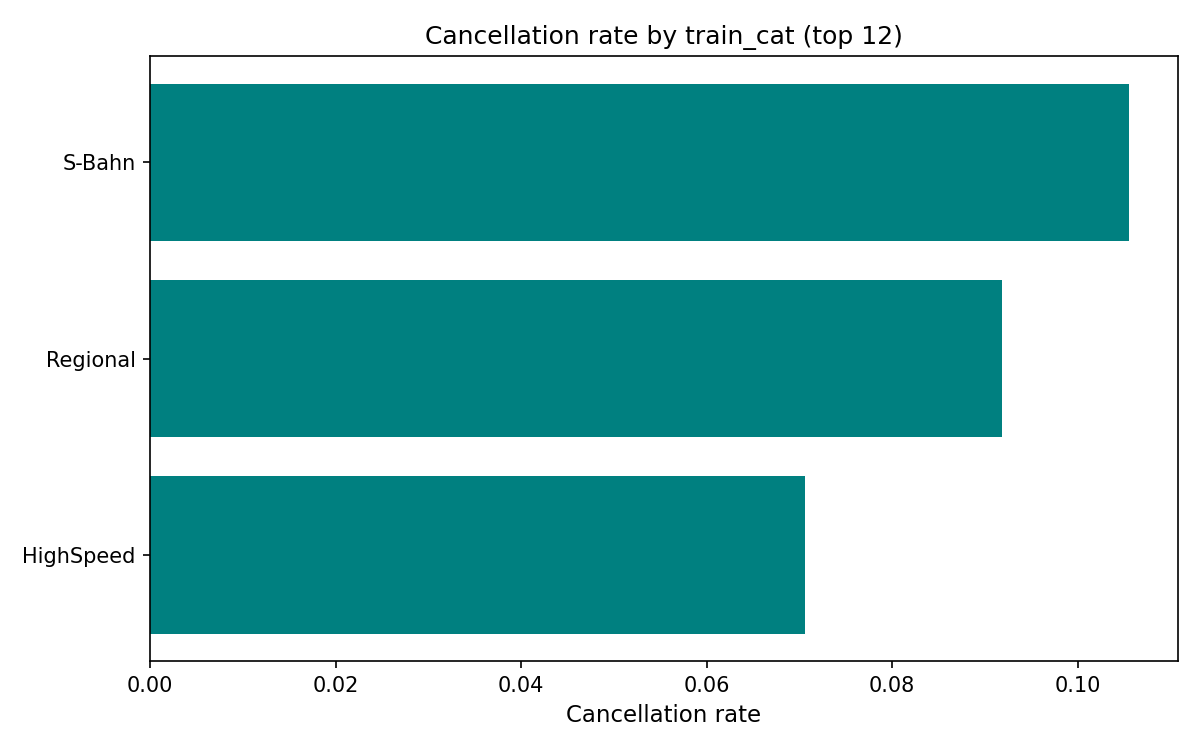
\includegraphics[width=\linewidth]{../../outputs/eda/cancel_rate_by_train_cat.png}
        \caption{Cancellation rate by \texttt{train\_cat}.}
    \end{subfigure}
    \hfill
    \begin{subfigure}[t]{0.48\textwidth}
        \centering
        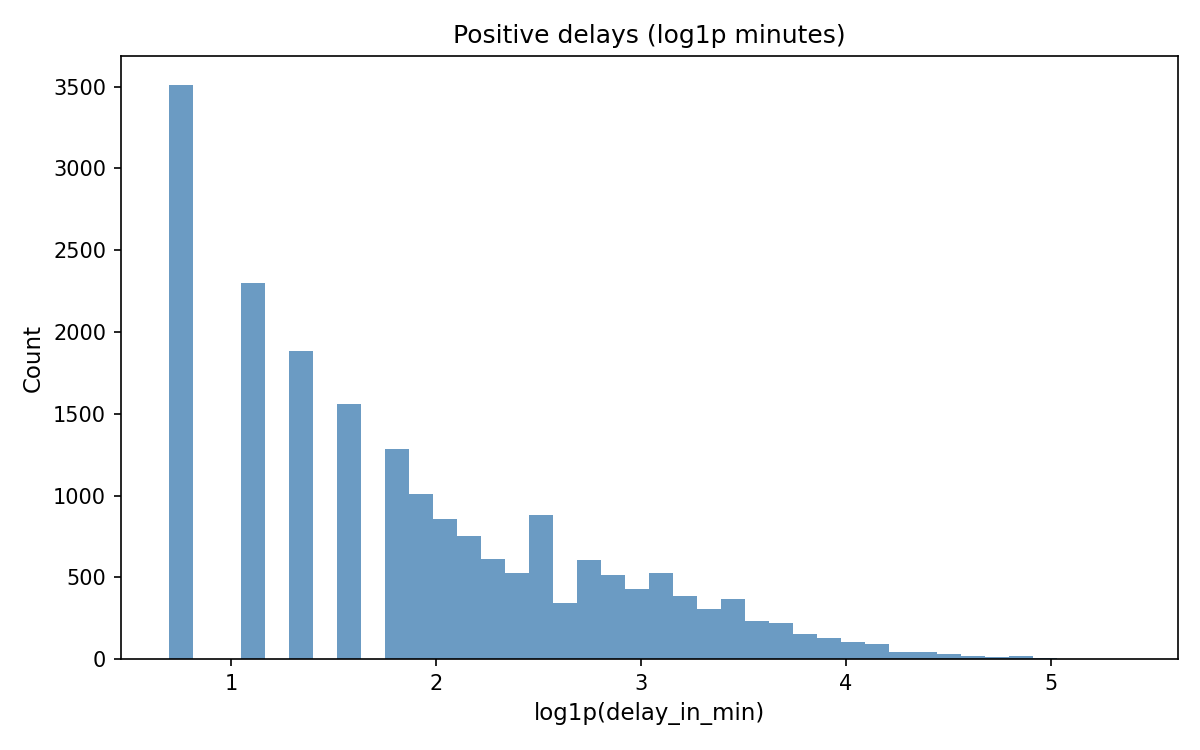
\includegraphics[width=\linewidth]{../../outputs/eda/delay_distribution_log1p.png}
        \caption{Positive-delay distribution on the log1p scale.}
    \end{subfigure}
    \caption{Compact exploratory overview of the Dortmund Hbf December 2025 data. The left panel motivates \texttt{train\_cat} as the exchangeable grouping factor, while the right panel motivates separating delay incidence from positive-delay magnitude.}
    \label{fig:eda_compact}
\end{figure}
\FloatBarrier

\subsection{From Phase 1 presentation to Phase 2 report focus}

The presentation associated with this project corresponded to an earlier Phase~1 analysis. In that version, the same three story lines were already present, but the main comparison focused on baseline versus hierarchical variants within one modeling family. For the written report, we revised the comparison so that the Bayesian alternatives would be more clearly distinct and the exchangeability assumption would be stated more explicitly. Accordingly, Phase~2 keeps the same dataset, substantive questions, and three stories, but shifts the primary comparison for binary outcomes to event-level Bernoulli versus grouped Binomial models, with \texttt{train\_cat} treated as the exchangeable grouping factor. The positive-delay log-normal models are retained as support models for delay magnitude rather than as the main comparison axis. Because Phase~2 changes both the comparison question and, for one model class, the observation unit, its numerical results are not expected to match Phase~1 exactly.

\section{Data}

The dataset consists of operational railway events observed at Dortmund Hauptbahnhof (Dortmund Hbf) during December 2025. The source used in this report is the project event table \texttt{Dortmund\_HBF\_December.csv}, where each row corresponds to one recorded stop event in the station timeline. This analysis table was produced by consolidating and cleaning raw operational event records for Dortmund Hbf in the project preprocessing pipeline into a single event-level file.

The unit of analysis is one train stop event. Some rows contain only arrival information, some only departure information, and some both. In total, the dataset contains 27{,}201 event rows, of which 16{,}205 contain arrival timestamps, 16{,}152 contain departure timestamps, and 5{,}156 contain both. The overall cancellation rate is 9.2\%, and the delay-incidence rate for delays greater than 0 minutes is 72.8\%. Among positive delays, the median delay is 5.0 minutes and the mean delay is 9.8 minutes. These summaries indicate that the project contains both binary outcomes and a right-skewed positive outcome component.

The three story lines are derived from the same event-level dataset. Story~1 uses cancellation incidence as the target, Story~2 uses arrival-delay incidence together with positive arrival-delay magnitude conditional on delay being greater than zero, and Story~3 uses departure-delay incidence together with positive departure-delay magnitude conditional on delay being greater than zero. This keeps the substantive setting fixed while allowing different outcome definitions across stories.

The main predictors describe temporal and categorical structure in the data, including weekday, hour, day of month, days until Christmas, train category / train type, and destination bucket. In the revised Phase~2 report, the multilevel grouping factor is represented by \texttt{train\_cat}. Destination information is reduced to a top-\(K\) representation with the remaining destinations grouped into an ``Other'' category in order to avoid an excessively sparse categorical expansion while preserving the most frequent stations.

Preprocessing was designed to align the data with the likelihood choices used later in the report. Binary targets were coded as 0/1 outcomes. Delay minutes were treated as non-negative, and the positive-delay component was modeled separately from the zero-delay component. This reflects the empirical structure seen in the exploratory analysis: cancellations are binary events, while delay magnitude is concentrated at zero with a positively skewed right tail among delayed trains. The grouped Binomial benchmark used in Phase~2 is obtained by aggregating event-level binary outcomes into grouped counts for the grouped incidence models, whereas the Bernoulli formulation retains the original event-level unit of analysis.

For evaluation, the pipeline applies a deterministic whole-day holdout split in which events with \texttt{day\_of\_month \% 5 == 0} form the held-out test set and all remaining events form the training set. This yields common held-out event sets for fair event-level Bernoulli versus grouped Binomial comparison. The resulting test-set sizes are 5{,}316 events in Story~1, 2{,}840 in Story~2, and 2{,}849 in Story~3. For grouped models, aggregation is performed within each split so that grouped predictions are still evaluated on the same held-out event sets. The same underlying dataset is therefore used consistently across all stories in the revised Phase~2 report, where the primary comparison is event-level Bernoulli versus grouped Binomial incidence modeling.

\section{Models}
\subsection{Story overview}

The revised Phase~2 analysis keeps the same three substantive story lines as the earlier presentation, but changes the primary comparison for the binary outcomes:
\begin{itemize}
    \item Story~1 models cancellation incidence;
    \item Story~2 models arrival-delay incidence and, separately, positive arrival-delay magnitude conditional on delay being greater than zero;
    \item Story~3 models departure-delay incidence and, separately, positive departure-delay magnitude conditional on delay being greater than zero.
\end{itemize}

The main comparison in the report is therefore between two Bayesian formulations for binary incidence outcomes, while the positive-delay magnitude models play a supporting role for the interpretation of non-zero delay size.

The earlier Phase~1 presentation emphasized baseline-versus-hierarchical comparisons within the same general family, whereas the present report uses Phase~2 to compare two more clearly distinct Bayesian incidence formulations.

\begin{table}[t]
\centering
\caption{Model roles in the revised Phase~2 report.}
\label{tab:model_overview}
\begin{tabular}{llll}
\hline
Story & Model ID & Outcome type & Role \\
\hline
1 & 1E\_bern & Cancellation incidence & Main event-level model \\
1 & 1G\_binom & Grouped cancellation incidence & Coarse benchmark \\
2 & 2E\_delay & Arrival delay incidence & Main event-level model \\
2 & 2G\_delay & Grouped arrival delay incidence & Coarse benchmark \\
2 & 2M\_log & Positive arrival-delay magnitude & Support model \\
3 & 3E\_delay & Departure delay incidence & Main event-level model \\
3 & 3G\_delay & Grouped departure delay incidence & Coarse benchmark \\
3 & 3M\_log & Positive departure-delay magnitude & Support model \\
\hline
\end{tabular}
\end{table}

\subsection{Event-level Bernoulli incidence models}

The first incidence formulation keeps the original event-level unit of analysis. For each event \(i\), the binary outcome is modeled as
\[
y_i \sim \mathrm{Bernoulli}(p_i),
\qquad
\mathrm{logit}(p_i) = \eta_i ,
\]
with
\[
\eta_i = \alpha + x_i^\top \beta + u_{j[i]},
\qquad
u_j \sim \mathrm{Normal}(0, \sigma_{\texttt{train\_cat}}).
\]
In Story~1, \(y_i\) indicates whether the event is canceled. In Stories~2 and~3, \(y_i\) indicates whether the delay is positive, conditional on restricting the data to non-canceled arrivals or departures respectively. The linear predictor includes temporal and categorical structure, such as weekday, time information, days until Christmas, destination bucket where applicable, and the multilevel train-category term. This event-level Bernoulli formulation is the most direct model for the report's primary predictive target, since the target of interest is event-level incidence.

\subsection{Grouped Binomial incidence models}

The second incidence formulation aggregates event-level binary outcomes into grouped counts and models them with a Binomial likelihood. For grouped cell \(g\),
\[
y_g \sim \mathrm{Binomial}(n_g, p_g),
\qquad
\mathrm{logit}(p_g) = \eta_g ,
\]
where \(y_g\) is the number of events with the outcome of interest and \(n_g\) is the total number of events in the group. In Story~1, grouping uses weekday, three-hour time bin, \texttt{train\_cat}, and event-type strata. In Stories~2 and~3, grouped data are formed analogously for delay-incidence outcomes over weekday, three-hour time bin, and \texttt{train\_cat}. The grouped Binomial models are therefore a coarser benchmark to the event-level Bernoulli models: they target the same substantive incidence questions, but use aggregated observations rather than the original event-level unit. This difference in observation unit is important later for model comparison.

\subsection{Positive-delay log-normal support models}

For Stories~2 and~3, positive delay magnitude is modeled separately from delay incidence. Conditional on delay being strictly greater than zero, the support model is
\[
\log(d_i) \sim \mathrm{Normal}(\mu_i, \sigma),
\qquad
\mu_i = \alpha + x_i^\top \beta + u_{j[i]},
\qquad
u_j \sim \mathrm{Normal}(0, \sigma_{\texttt{train\_cat}}),
\]
where \(d_i\) is positive delay in minutes. This separates the question ``does a delay occur?'' from the question ``how large is the delay if it occurs?'' The specification follows the strong empirical right-skew of positive delays seen in the exploratory analysis and keeps the positive-delay models as support models rather than the main comparison axis of the report.

\subsection{Exchangeability and multilevel structure}

A central feature of the revised report is that the grouping factor is made explicit. The exchangeable multilevel grouping factor is \texttt{train\_cat}. Its levels are treated as exchangeable in the sense that the corresponding category-specific effects are modeled as draws from a common group-level distribution rather than estimated independently without pooling. This partial-pooling structure allows the models to share information across train categories while still permitting category-specific deviations from the global mean structure. The exchangeability assumption is substantively reasonable because the train categories represent related operational classes that are different but not unrelated. In the results sections, this structure is examined through posterior group-effect summaries and posterior category probabilities by \texttt{train\_cat}.

\section{Priors}

The report uses explicit proper priors for all fitted models in order to satisfy the project requirements and to ensure that regularization is transparent rather than inherited from software defaults. The prior design follows three simple principles: regression effects are centered at zero, intercepts are centered at story-specific baseline values on the link scale, and group-level variation is controlled through a positive prior on the shared scale of the exchangeable \texttt{train\_cat} effects. This is consistent with the course emphasis that priors should be explicit, proper, scale-aware, and aligned with model structure.

For the event-level Bernoulli and grouped Binomial incidence models, continuous predictor coefficients use \(\mathrm{Normal}(0, 0.5)\), and fixed categorical effects also use \(\mathrm{Normal}(0, 0.5)\). The story-specific intercept priors are \(\mathrm{Normal}(\mu, 0.7)\), with \(\mu=-2.2\) for Story~1 cancellation incidence, \(\mu=1.4\) for Story~2 arrival-delay incidence, and \(\mu=0.85\) for Story~3 departure-delay incidence. The group-level standard deviation for exchangeable \texttt{train\_cat} effects uses \(\mathrm{HalfNormal}(0.35)\). In implementation, Bernoulli and grouped Binomial incidence models share the same prior scales within each story so that the primary comparison is not driven by different prior strength across incidence formulations.

For the positive-delay magnitude models, the response is modeled on the log-delay scale. Continuous coefficients again use \(\mathrm{Normal}(0, 0.5)\), and fixed categorical effects use \(\mathrm{Normal}(0, 0.5)\). The intercept prior is \(\mathrm{Normal}(1.5, 0.8)\). The group-level standard deviation for exchangeable \texttt{train\_cat} effects again uses \(\mathrm{HalfNormal}(0.35)\), and the residual standard deviation uses \(\mathrm{HalfNormal}(0.7)\). This keeps the overall regularization logic parallel to the incidence models while allowing residual spread on the log-magnitude scale.

These priors are weakly informative rather than flat: zero-centered effects encode ``no effect'' as the default, while moderate scales still permit substantial updating from the data. The separate intercept locations reflect baseline prevalence differences between cancellations and delays, and the shared group-level scale reflects the exchangeability assumption for \texttt{train\_cat}. The prior specification was intentionally kept parallel across the two incidence model classes so that the Bernoulli-versus-Binomial comparison primarily reflects modeling formulation and observation unit rather than arbitrary differences in prior regularization. A formal wider-prior sensitivity rerun was not included in the final Phase~2 pipeline, so prior robustness is discussed later as a limitation rather than presented as a completed result.

\section{Code and implementation}

The analysis was implemented as a modular Python pipeline with \texttt{run\_project.py} as the command-line entry point and \texttt{pipeline.py} as the main workflow driver. Supporting modules handle data preparation, feature construction, model building, evaluation, and plotting. The pipeline runs the revised Phase~2 analysis end to end, producing summaries, prior and posterior predictive plots, calibration artifacts, holdout comparison outputs, and PSIS-LOO diagnostics. For the final report run, the sampling configuration used 4 chains, 2000 posterior draws per chain, 2000 tuning iterations per chain, and target acceptance 0.95. The full source code is submitted separately as a repository or zip archive, as required by the course instructions.

\section{Convergence diagnostics}

Posterior computation was assessed using standard MCMC diagnostics before interpreting posterior summaries or predictive comparisons. The main checks were trace plots, the potential scale reduction factor \(\hat{R}\), effective sample size (ESS), and the number of divergent transitions. Across the main incidence models, divergences were 0, the largest reported \(\hat{R}\) was 1.000, and the smallest reported bulk ESS was 1560.40. The positive-delay magnitude support models were also stable, with 0 divergences, maximum \(\hat{R}=1.000\), and minimum bulk ESS 1759.75. Selected trace plots are provided in Appendix~\ref{sec:appendix_diagnostics}, consistent with the course guidance that lower-priority diagnostic details may be moved to the appendix.

\section{Model comparison}

\subsection{Comparison principle}

The main Phase~2 comparison is between two Bayesian incidence formulations for the same substantive binary questions: an event-level Bernoulli model and a grouped Binomial benchmark. Both incorporate the same exchangeable grouping factor, \texttt{train\_cat}, but they differ in observation unit. We therefore compare them on the same held-out event sets, which matches the report's event-level predictive target.

\subsection{Why direct PSIS-LOO was not used for the main incidence comparison}

We do not use direct PSIS-LOO ranking to compare the Bernoulli and grouped Binomial incidence models, because they factorize the likelihood over different observation units. The event-level models use individual events, whereas the grouped models use aggregated counts. For that reason, direct Bernoulli-versus-Binomial PSIS-LOO comparison is not appropriate here. We still compute PSIS-LOO and Pareto-\(k\) summaries for each fitted model individually to verify that those LOO estimates are numerically stable.

\subsection{Held-out event-level comparison}

Because our substantive target is event-level incidence prediction, we compare the candidate incidence models on common held-out event sets. We use two proper scoring rules, Brier score and log loss, so that both formulations are judged on the same predictive task even though one of them is fitted on grouped data.

\begin{figure}[t]
    \centering
    \begin{subfigure}[t]{0.48\textwidth}
        \centering
        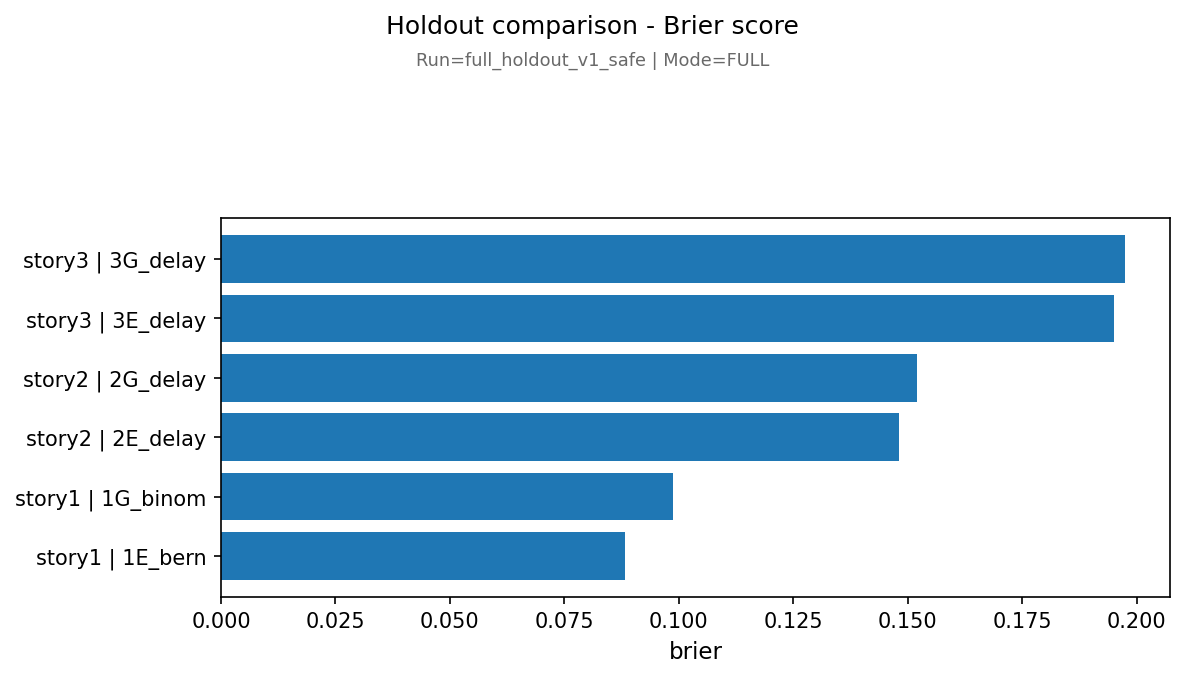
\includegraphics[width=\linewidth]{../../outputs/ppc/holdout_brier_comparison.png}
        \caption{Held-out Brier score. Lower is better.}
    \end{subfigure}
    \hfill
    \begin{subfigure}[t]{0.48\textwidth}
        \centering
        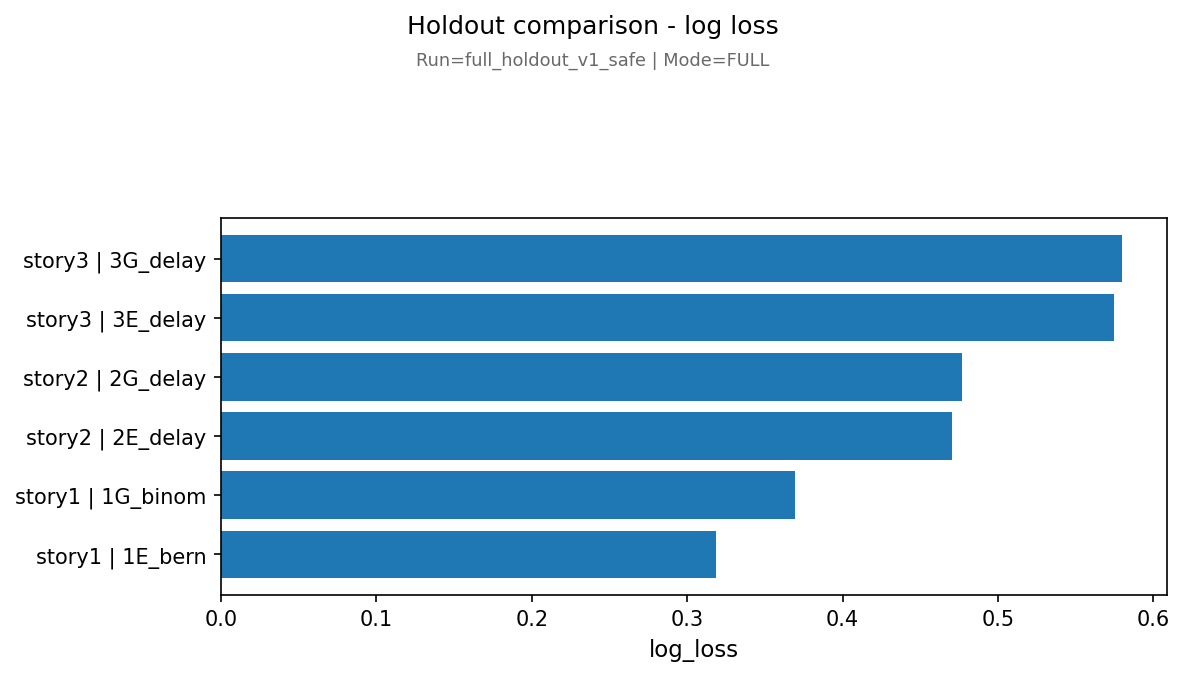
\includegraphics[width=\linewidth]{../../outputs/ppc/holdout_log_loss_comparison.png}
        \caption{Held-out log loss. Lower is better.}
    \end{subfigure}
    \caption{Primary Phase~2 incidence comparison on common held-out event sets. Across all three stories, the event-level Bernoulli models outperform the grouped Binomial benchmarks.}
    \label{fig:holdout_compact}
\end{figure}

\subsection{Story-by-story comparison result}

The held-out comparison gives a consistent ranking across all three incidence stories:
\begin{itemize}
    \item Story~1: \texttt{1E\_bern} clearly outperformed \texttt{1G\_binom} on both metrics (log loss \(0.3186\) vs \(0.3693\); Brier \(0.0882\) vs \(0.0987\));
    \item Story~2: \texttt{2E\_delay} again outperformed \texttt{2G\_delay}, with a moderate margin (log loss \(0.4702\) vs \(0.4770\); Brier \(0.1481\) vs \(0.1521\));
    \item Story~3: the comparison was closest, but \texttt{3E\_delay} still performed better than \texttt{3G\_delay} on both metrics (log loss \(0.5749\) vs \(0.5798\); Brier \(0.1952\) vs \(0.1974\)).
\end{itemize}

\begin{table}[t]
\centering
\caption{Summary of the main held-out incidence comparison in Phase~2.}
\label{tab:comparison_summary}
\begin{tabular}{llll}
\hline
Story & Event model & Grouped model & Main conclusion \\
\hline
1 & 1E\_bern & 1G\_binom & Bernoulli clearly better \\
2 & 2E\_delay & 2G\_delay & Bernoulli moderately better \\
3 & 3E\_delay & 3G\_delay & Bernoulli slightly better \\
\hline
\end{tabular}
\end{table}

Across stories, the pattern is stable: grouped Binomial models are useful coarse benchmarks, but event-level Bernoulli models are the predictive winners on common held-out event sets.

\section{Model checks and predictive performance}
\subsection{Prior predictive checks}

We use prior predictive checks for the main event-level incidence models to confirm that the chosen priors generate plausible baseline event rates before seeing the data. Across all three stories, the observed rates fall within reasonable prior predictive ranges, which supports the use of weakly informative, scale-aware priors rather than overly diffuse or overly restrictive ones.

\begin{figure}[t]
    \centering
    \begin{subfigure}[t]{0.32\textwidth}
        \centering
        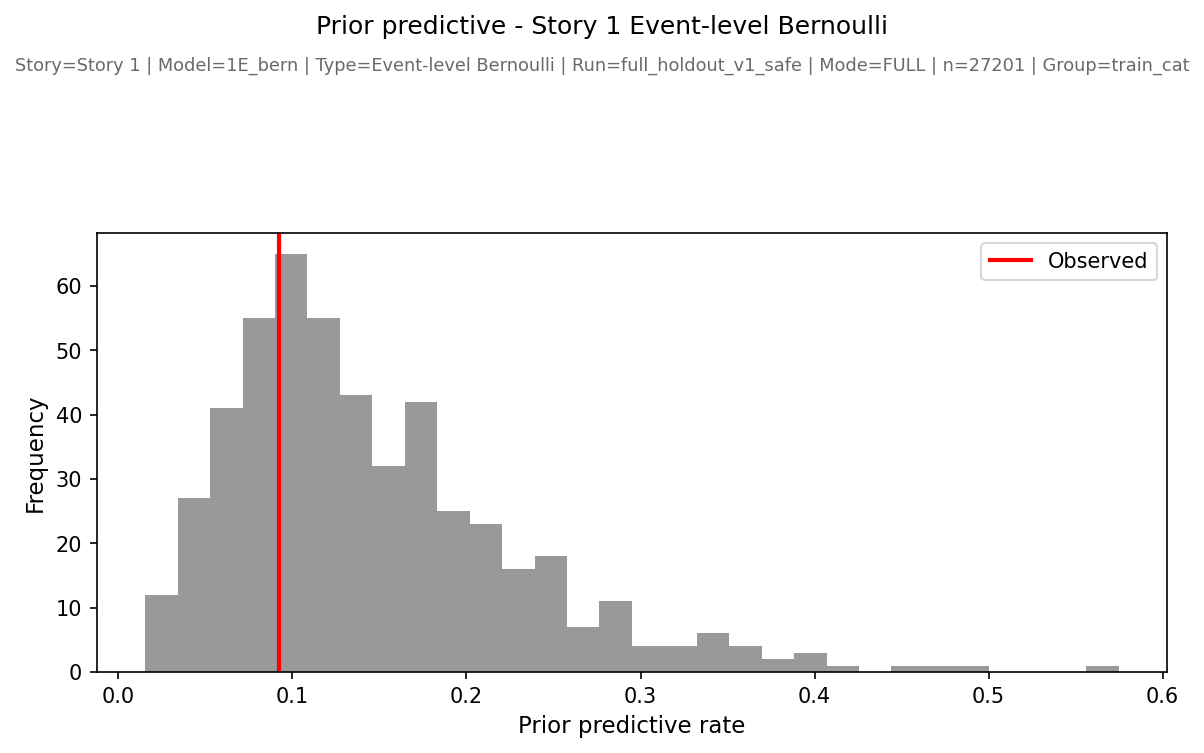
\includegraphics[width=\linewidth]{../../outputs/ppc/prior_1E_bern.png}
        \caption{Story 1}
    \end{subfigure}
    \hfill
    \begin{subfigure}[t]{0.32\textwidth}
        \centering
        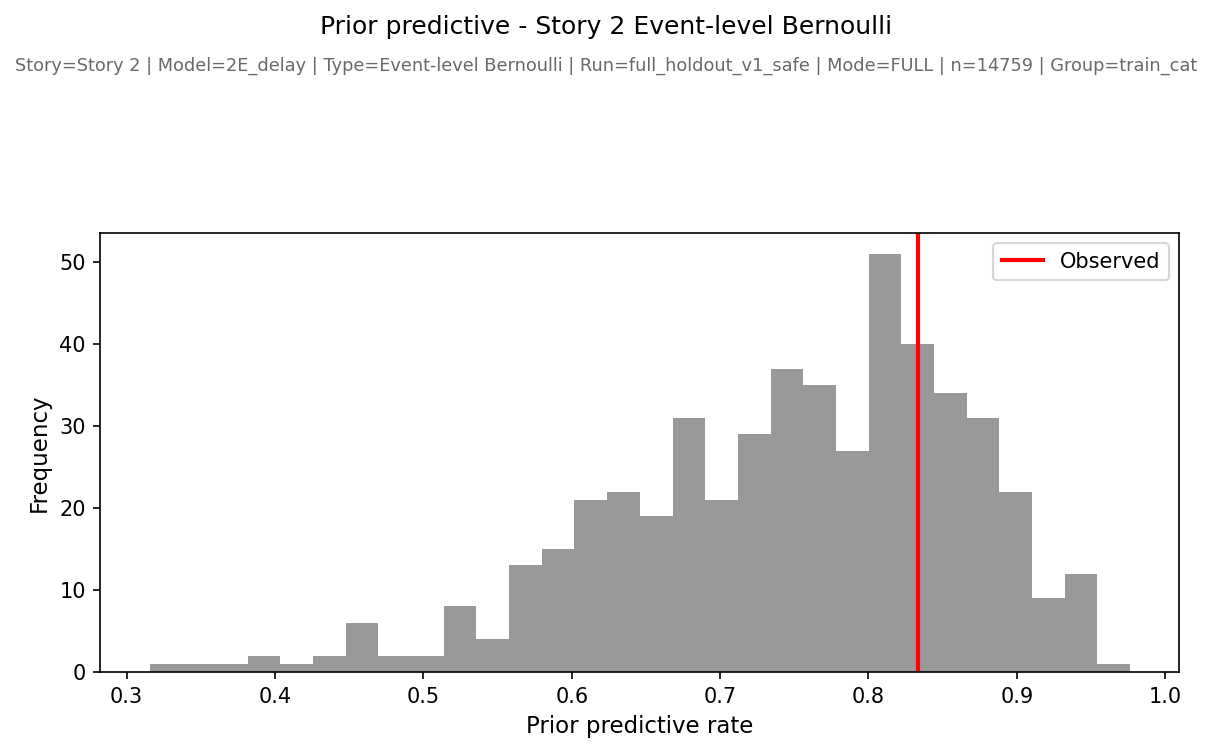
\includegraphics[width=\linewidth]{../../outputs/ppc/prior_2E_delay.png}
        \caption{Story 2}
    \end{subfigure}
    \hfill
    \begin{subfigure}[t]{0.32\textwidth}
        \centering
        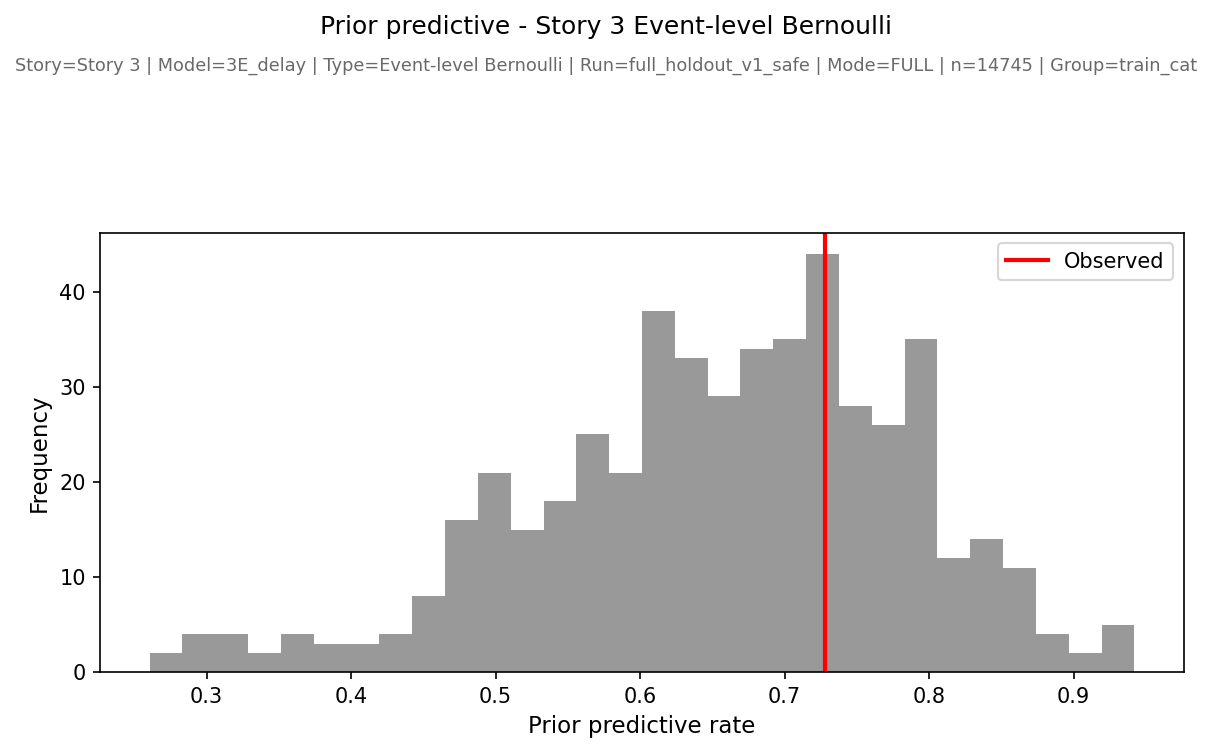
\includegraphics[width=\linewidth]{../../outputs/ppc/prior_3E_delay.png}
        \caption{Story 3}
    \end{subfigure}
    \caption{Prior predictive checks for the main event-level incidence models. The observed event rates fall within plausible prior predictive ranges in all three stories.}
    \label{fig:prior_compact}
\end{figure}

\subsection{Posterior predictive checks}

The posterior predictive checks show that the fitted models reproduce the main empirical structure relevant to each outcome type. For incidence, both the event-level Bernoulli and grouped Binomial formulations reproduce the overall event-rate pattern, with the grouped PPCs interpreted after the corrected weighted-rate construction. For positive-delay magnitude, the log-normal support models capture the main right-skewed bulk of the positive-delay distribution, although the extreme upper tail is less fully assessed.

\begin{figure}[!b]
    \centering
    \captionsetup{font=small}
    \begin{subfigure}[t]{0.40\textwidth}
        \centering
        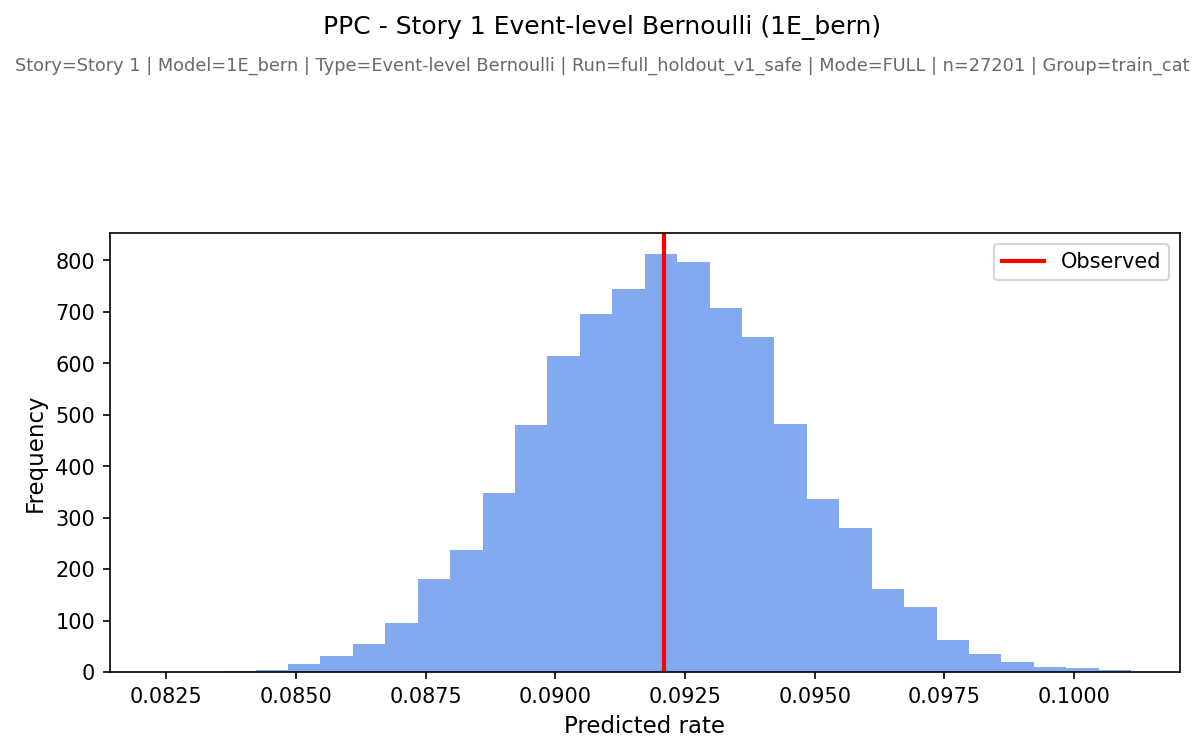
\includegraphics[width=\linewidth]{../../outputs/ppc/ppc_1E_bern.png}
        \caption{Story 1 event-level Bernoulli}
    \end{subfigure}
    \hfill
    \begin{subfigure}[t]{0.40\textwidth}
        \centering
        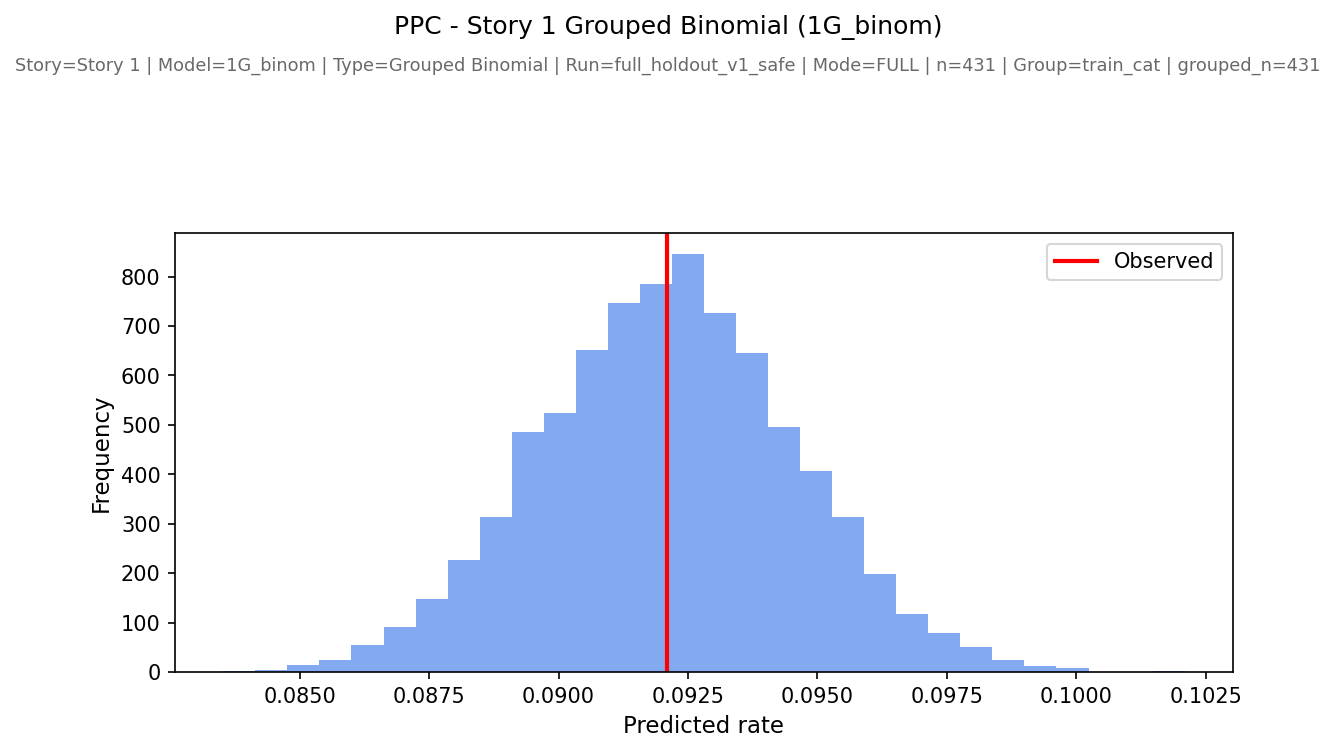
\includegraphics[width=\linewidth]{../../outputs/ppc/ppc_1G_binom.png}
        \caption{Story 1 grouped Binomial}
    \end{subfigure}

    \vspace{0.15em}

    \begin{subfigure}[t]{0.40\textwidth}
        \centering
        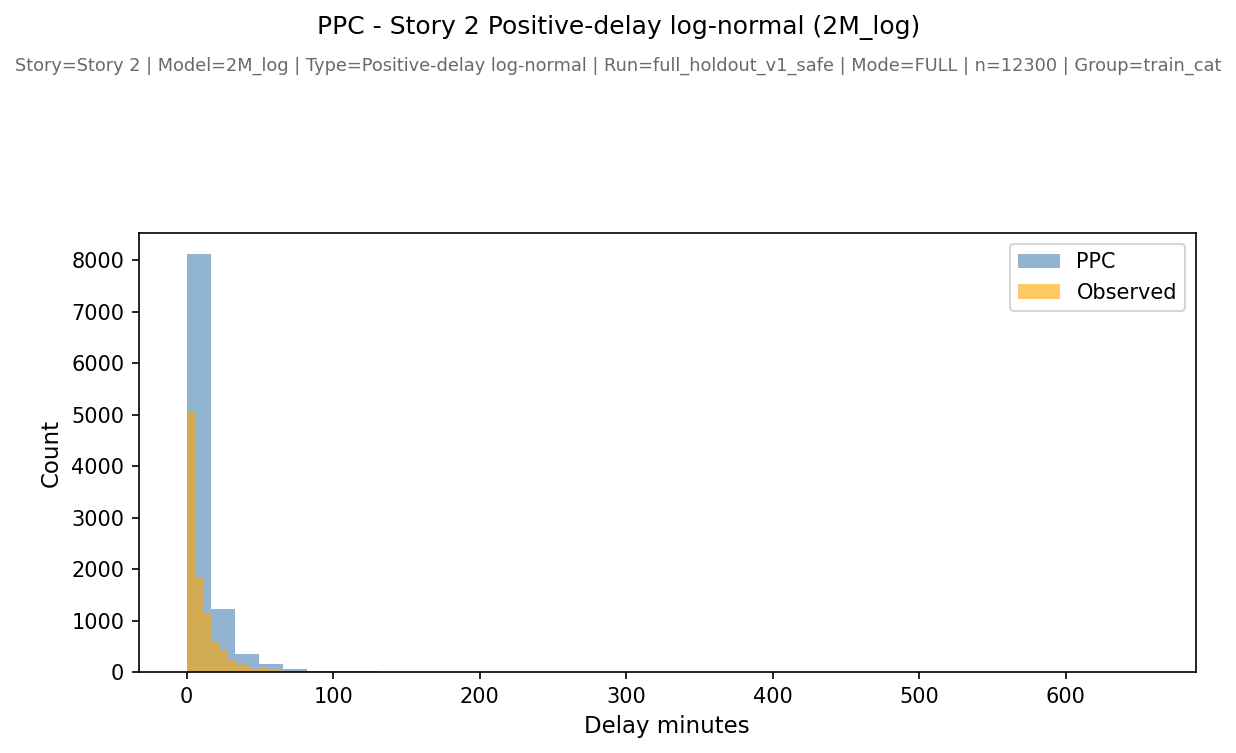
\includegraphics[width=\linewidth]{../../outputs/ppc/ppc_2M_log.png}
        \caption{Story 2 positive-delay magnitude}
    \end{subfigure}
    \hfill
    \begin{subfigure}[t]{0.40\textwidth}
        \centering
        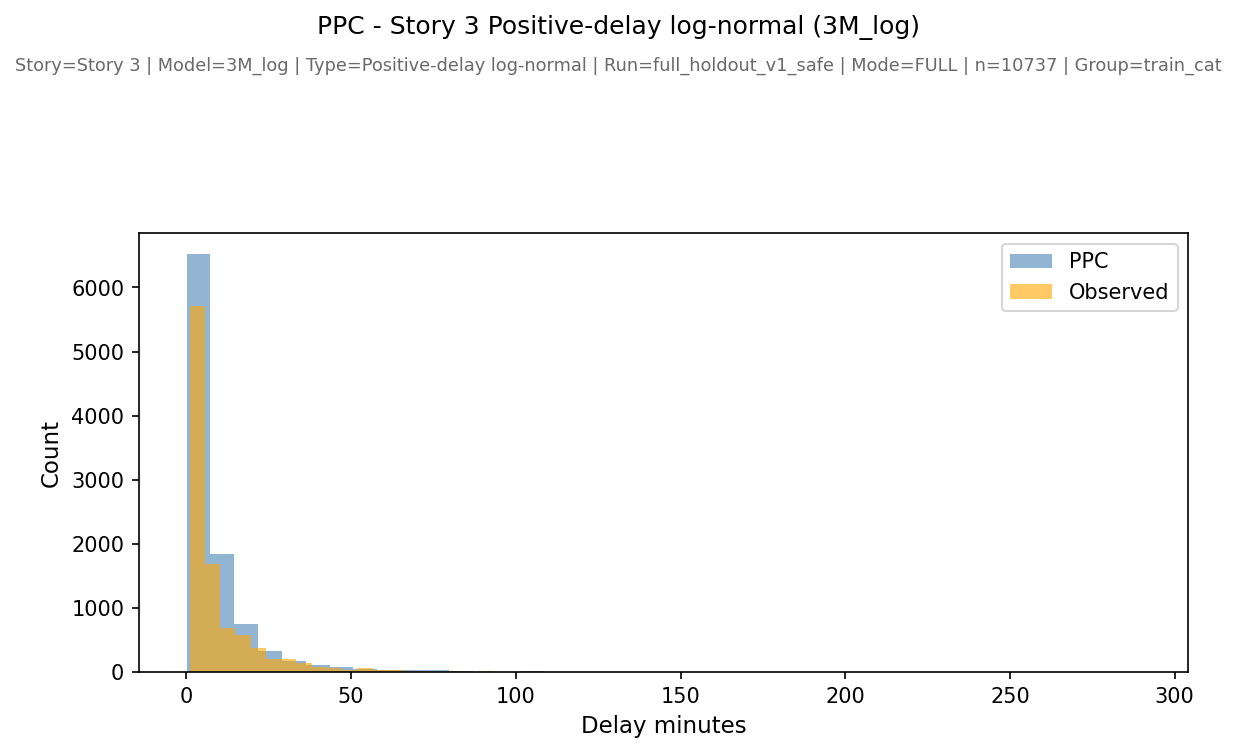
\includegraphics[width=\linewidth]{../../outputs/ppc/ppc_3M_log.png}
        \caption{Story 3 positive-delay magnitude}
    \end{subfigure}
    \caption{Compact posterior predictive checks. The top row compares event-level and grouped incidence PPCs in Story~1, while the bottom row summarizes the bulk fit of the positive-delay support models for Stories~2 and~3.}
    \label{fig:ppc_compact}
\end{figure}

\subsection{Calibration}

Calibration complements overall scoring by checking whether predicted probabilities agree with empirical frequencies on held-out events. Story~1 provides the clearest visual contrast: the event-level Bernoulli model calibrates better and yields a cleaner separation of the exchangeable \texttt{train\_cat} effects than the grouped Binomial benchmark. Stories~2 and~3 show the same overall direction more moderately, with both grouped models remaining usable coarse benchmarks but the event-level Bernoulli models staying at least as well calibrated and preserving clearer category-level structure.

\begin{figure}[t]
    \centering
    \captionsetup{font=small}
    \begin{subfigure}[t]{0.40\textwidth}
        \centering
        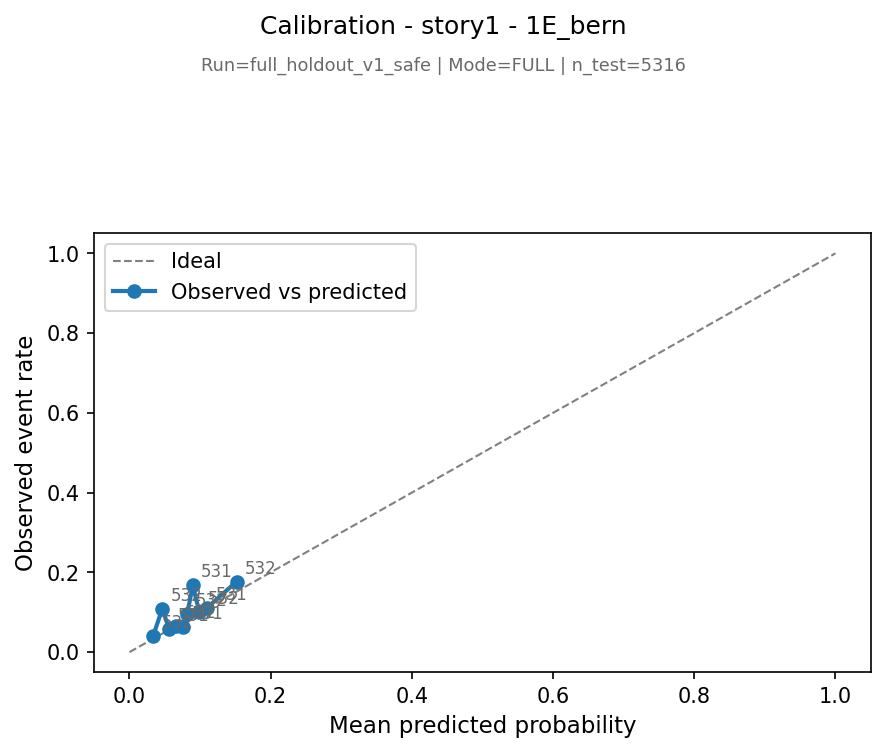
\includegraphics[width=\linewidth]{../../outputs/ppc/story1_calibration_1E_bern.png}
        \caption{Story~1 calibration: event-level Bernoulli}
    \end{subfigure}
    \hfill
    \begin{subfigure}[t]{0.40\textwidth}
        \centering
        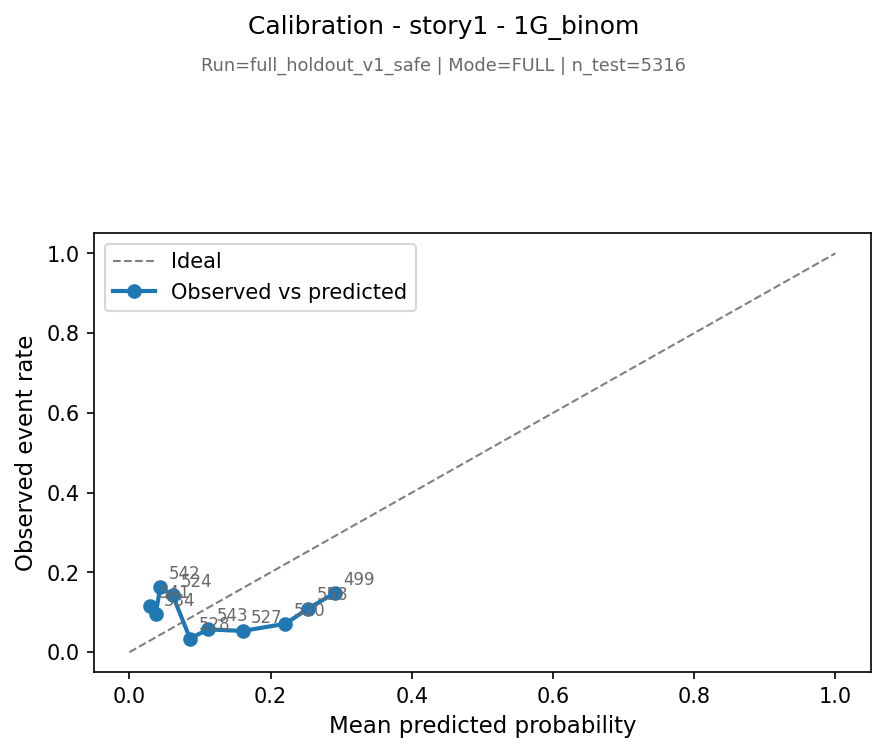
\includegraphics[width=\linewidth]{../../outputs/ppc/story1_calibration_1G_binom.png}
        \caption{Story~1 calibration: grouped Binomial}
    \end{subfigure}

    \vspace{0.15em}

    \begin{subfigure}[t]{0.40\textwidth}
        \centering
        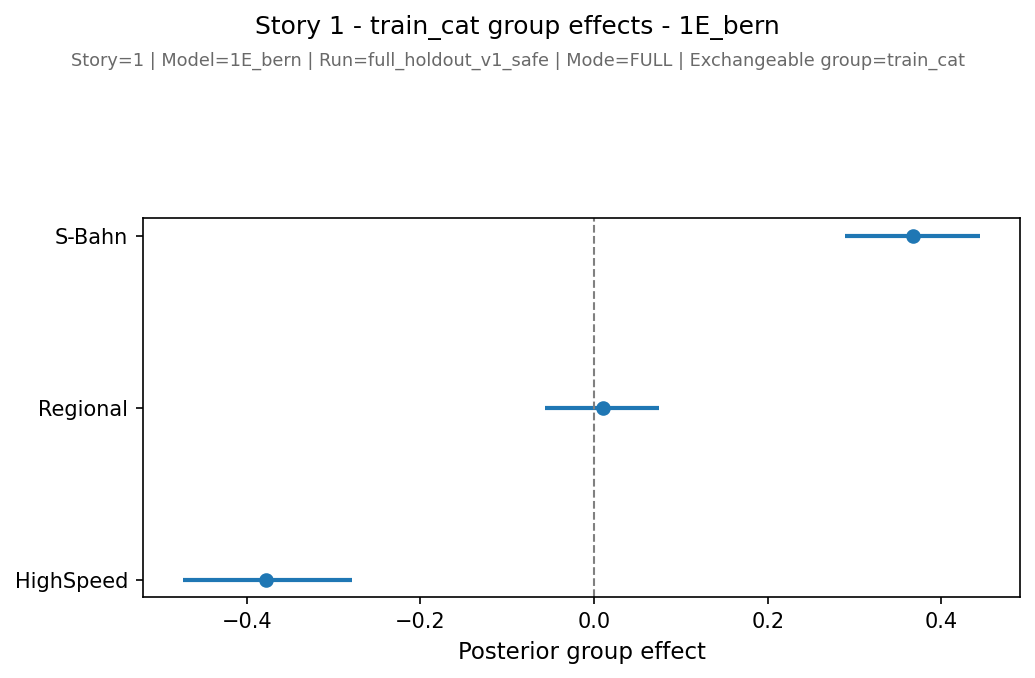
\includegraphics[width=\linewidth]{../../outputs/ppc/story1_train_cat_effects_1E_bern.png}
        \caption{Story~1 \texttt{train\_cat} effects: event-level Bernoulli}
    \end{subfigure}
    \hfill
    \begin{subfigure}[t]{0.40\textwidth}
        \centering
        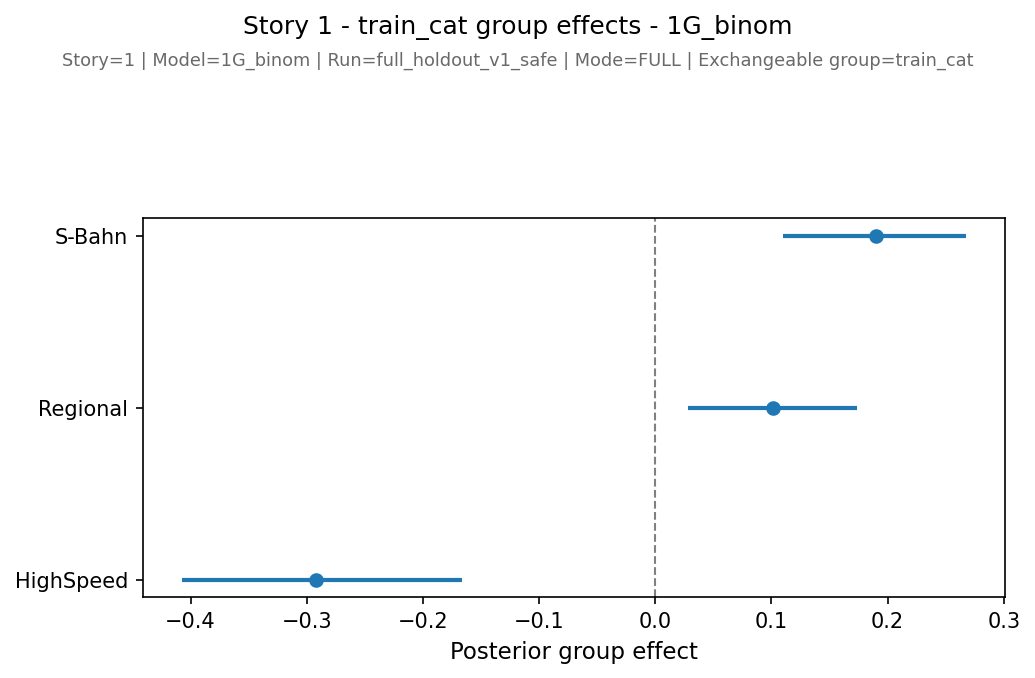
\includegraphics[width=\linewidth]{../../outputs/ppc/story1_train_cat_effects_1G_binom.png}
        \caption{Story~1 \texttt{train\_cat} effects: grouped Binomial}
    \end{subfigure}
    \caption{Compact Story~1 diagnostics. The event-level Bernoulli model calibrates better and yields a cleaner separation of the exchangeable \texttt{train\_cat} effects than the grouped Binomial benchmark.}
    \label{fig:story1_compact}
\end{figure}

\FloatBarrier

\subsection{Held-out predictive performance}

Held-out event-level predictive performance provides the final external check on the comparison. As shown in Figure~\ref{fig:holdout_compact}, the event-level Bernoulli formulation outperforms the grouped Binomial benchmark on common held-out event sets under both Brier score and log loss. The magnitude of the advantage differs by story: strongest for cancellation incidence in Story~1, smaller but clear for arrival-delay incidence in Story~2, and narrow but consistent for departure-delay incidence in Story~3.

Taken together with prior checks, posterior predictive checks, and calibration behavior, this supports the same overall interpretation: grouped Binomial models are useful coarse benchmarks, but event-level Bernoulli models provide the best combination of plausibility, calibration, and held-out predictive accuracy for the incidence stories.

\section{Limitations and potential improvements}

Several limitations should be kept in mind. The grouped Binomial models are intentionally coarser than the event-level Bernoulli models because they use aggregated counts rather than the original event-level observations, so the Phase~2 comparison is not a pure likelihood-only contrast with all other features held fixed. The positive-delay log-normal models also play a supporting role rather than serving as the main comparison axis, so our strongest conclusions concern incidence rather than positive-delay magnitude. In addition, the predictive comparison is based on a single held-out split rather than repeated blocked validation. Natural next steps would therefore include repeated blocked holdout evaluation, richer temporal structure, and more tail-focused checks for the positive-delay support models, but these extensions would not change the main Phase~2 incidence conclusion.

\section{Conclusion}

This report studied operational railway events at Dortmund Hbf in December 2025 through three related story lines: cancellation incidence, arrival-delay incidence with positive-delay magnitude, and departure-delay incidence with positive-delay magnitude. The revised Phase~2 analysis focused on a clear comparison between two Bayesian incidence formulations, namely event-level Bernoulli models and grouped Binomial benchmarks, while treating \texttt{train\_cat} as the exchangeable multilevel grouping factor. Positive-delay log-normal models were retained as support models for the magnitude of non-zero delays rather than as the main comparison axis.

The final result is consistent across all three incidence stories. Event-level Bernoulli models achieved better predictive performance than grouped Binomial benchmarks in every story, with the advantage strongest for cancellation incidence in Story~1, smaller but still clear for arrival-delay incidence in Story~2, and narrow but consistent for departure-delay incidence in Story~3. Together with calibration and posterior predictive checks, these results support the conclusion that the event-level Bernoulli formulation is the preferred strategy for this report's event-level predictive target, while grouped Binomial models remain useful coarse benchmarks.


\FloatBarrier
\clearpage
\begin{thebibliography}{9}
\bibitem{db_data_2025}
Deutsche Bahn operational event records for Dortmund Hbf (December 2025), processed into the project event table \texttt{Dortmund\_HBF\_December.csv}.

\bibitem{pymc}
Salvatier, J., Wiecki, T. V., and Fonnesbeck, C. (2016).
Probabilistic programming in Python using PyMC3.
\textit{PeerJ Computer Science}, 2:e55.

\bibitem{arviz}
Kumar, R., Carroll, C., Hartikainen, A., and Martin, O. (2019).
ArviZ a unified library for exploratory analysis of Bayesian models in Python.
\textit{Journal of Open Source Software}, 4(33), 1143.

\bibitem{vehtari2017}
Vehtari, A., Gelman, A., and Gabry, J. (2017).
Practical Bayesian model evaluation using leave-one-out cross-validation and WAIC.
\textit{Statistics and Computing}, 27, 1413--1432.
\end{thebibliography}

\FloatBarrier
\clearpage
\appendix
\FloatBarrier
\section{Appendix}

\subsection{Additional exploratory data analysis}
\label{sec:appendix_eda}
\FloatBarrier

\begin{figure}[htbp]
    \centering
    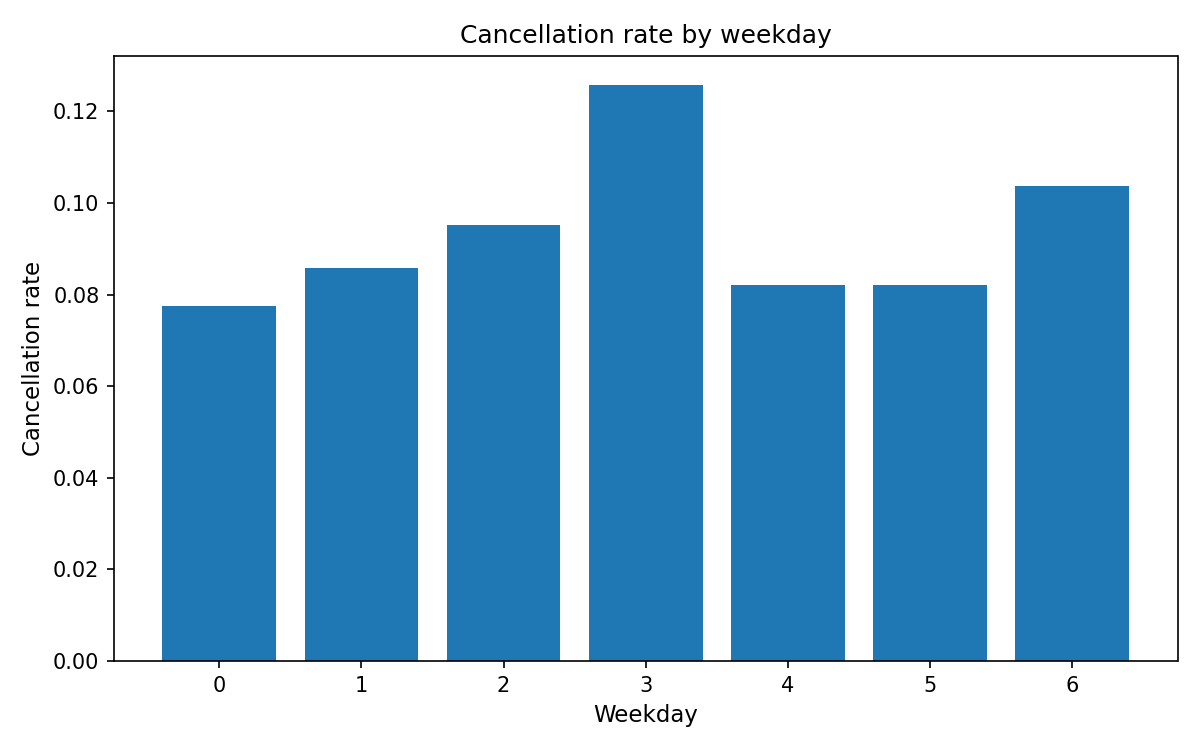
\includegraphics[width=0.72\textwidth]{../../outputs/eda/cancel_rate_by_weekday.png}
    \caption{Additional exploratory view: cancellation rate by weekday.}
    \label{fig:appendix_cancel_weekday}
\end{figure}

\begin{figure}[htbp]
    \centering
    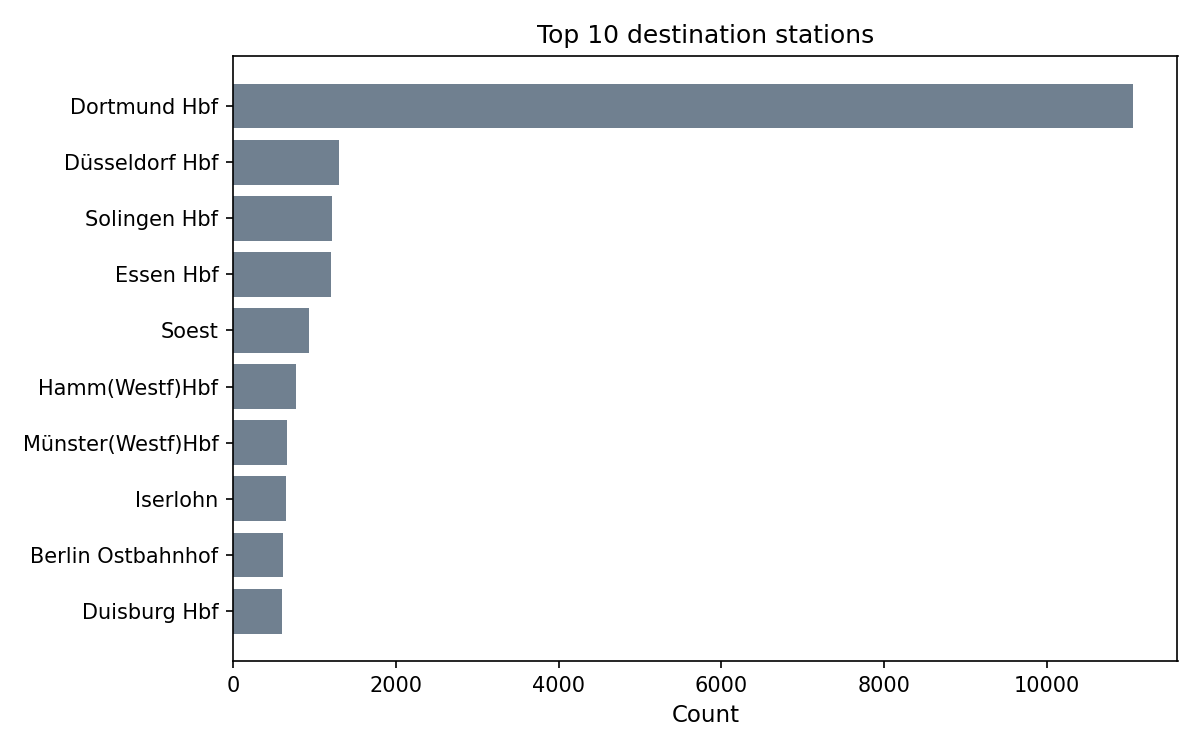
\includegraphics[width=0.72\textwidth]{../../outputs/eda/top_destinations.png}
    \caption{Additional exploratory view: top destination stations.}
    \label{fig:appendix_top_destinations}
\end{figure}

\FloatBarrier
\clearpage
\subsection{Additional sampler diagnostics}
\label{sec:appendix_diagnostics}
\FloatBarrier

Selected trace plots are placed in the appendix because the main text reports convergence through summary diagnostics, while the detailed chain-level evidence is lower-priority supporting material.

\subsubsection*{Story 1 incidence models}

\begin{figure}[htbp]
    \centering
    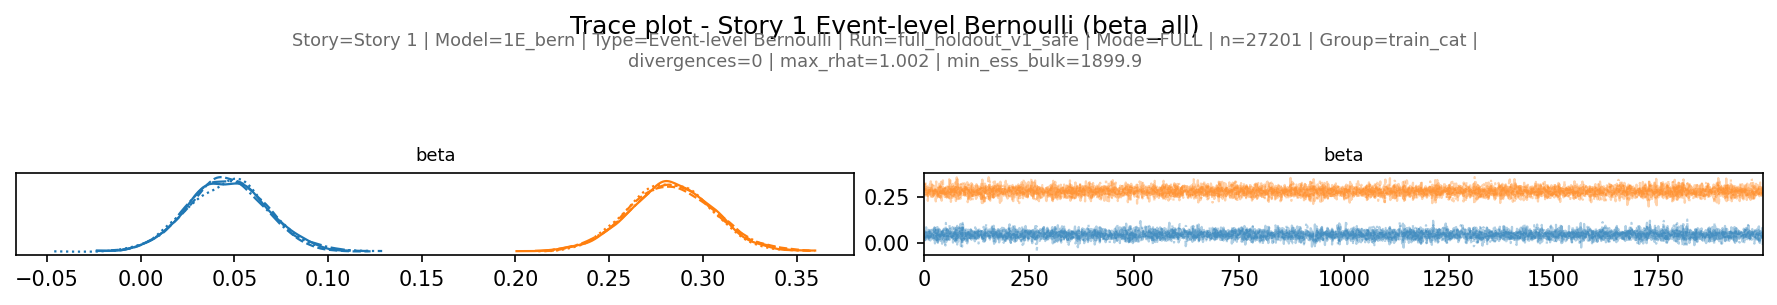
\includegraphics[width=0.8\textwidth]{../../outputs/models/trace_1E_bern_beta_all.png}
    \caption{Trace plot for Story 1 event-level Bernoulli: \texttt{beta\_all}.}
    \label{fig:trace_1E_beta}
\end{figure}

\begin{figure}[htbp]
    \centering
    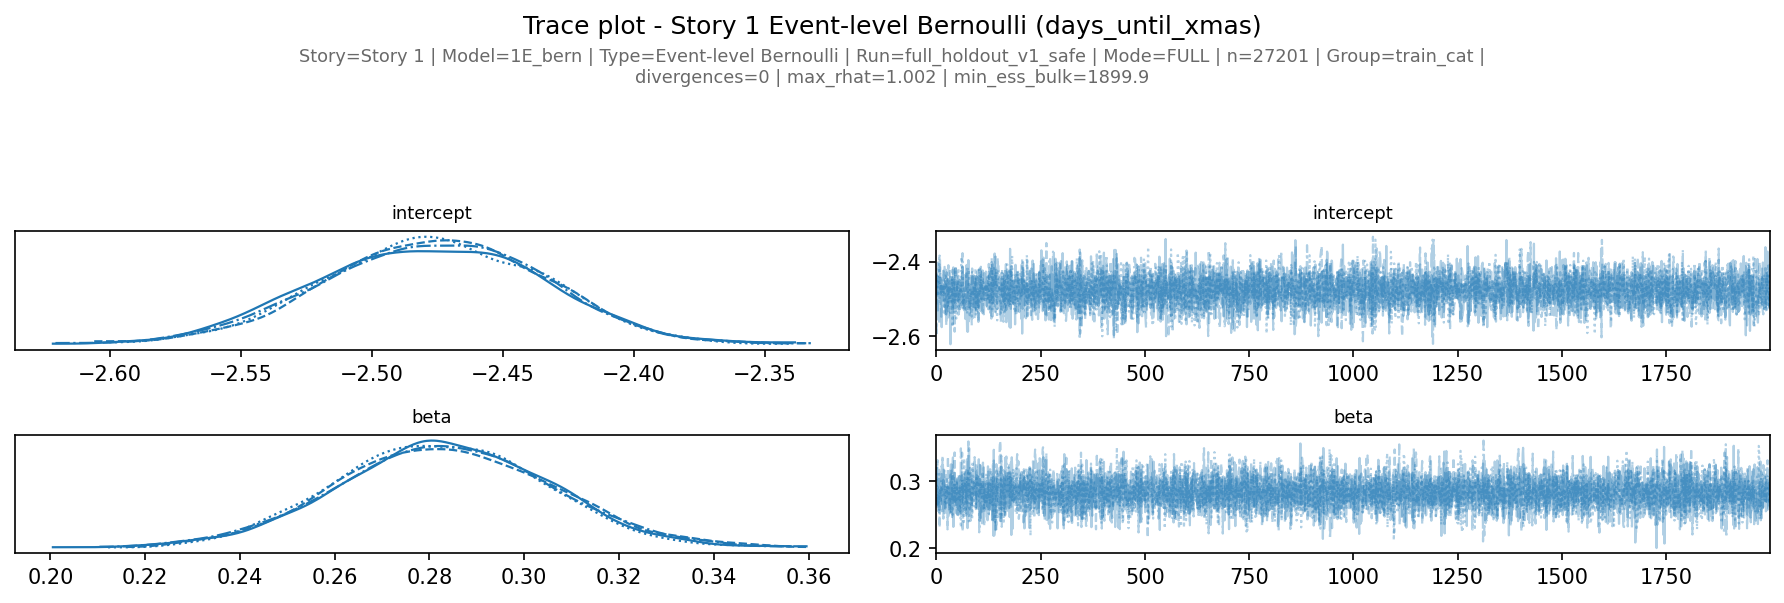
\includegraphics[width=0.8\textwidth]{../../outputs/models/trace_1E_bern_days_until_xmas.png}
    \caption{Trace plot for Story 1 event-level Bernoulli: \texttt{days\_until\_xmas}.}
    \label{fig:trace_1E_days}
\end{figure}

\begin{figure}[htbp]
    \centering
    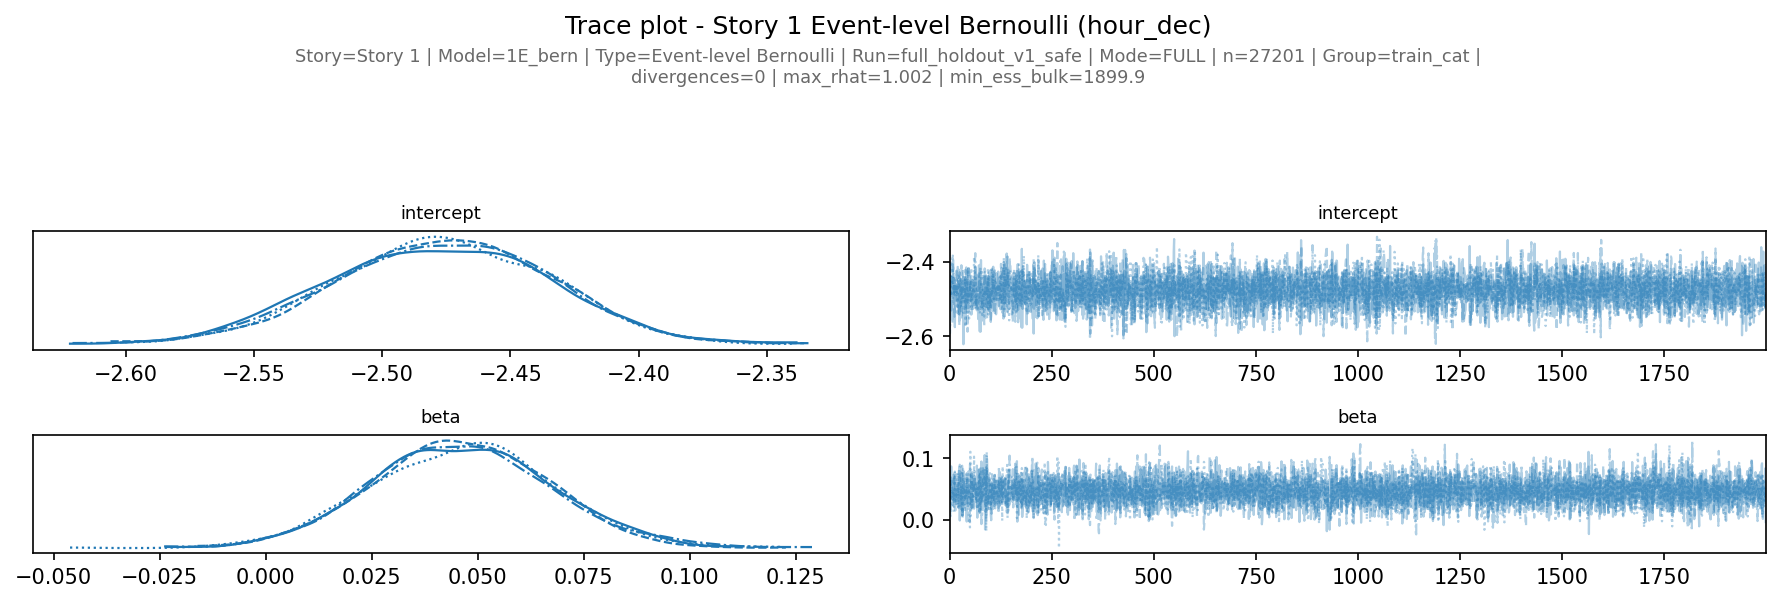
\includegraphics[width=0.8\textwidth]{../../outputs/models/trace_1E_bern_hour_dec.png}
    \caption{Trace plot for Story 1 event-level Bernoulli: \texttt{hour\_dec}.}
    \label{fig:trace_1E_hour}
\end{figure}

\begin{figure}[htbp]
    \centering
    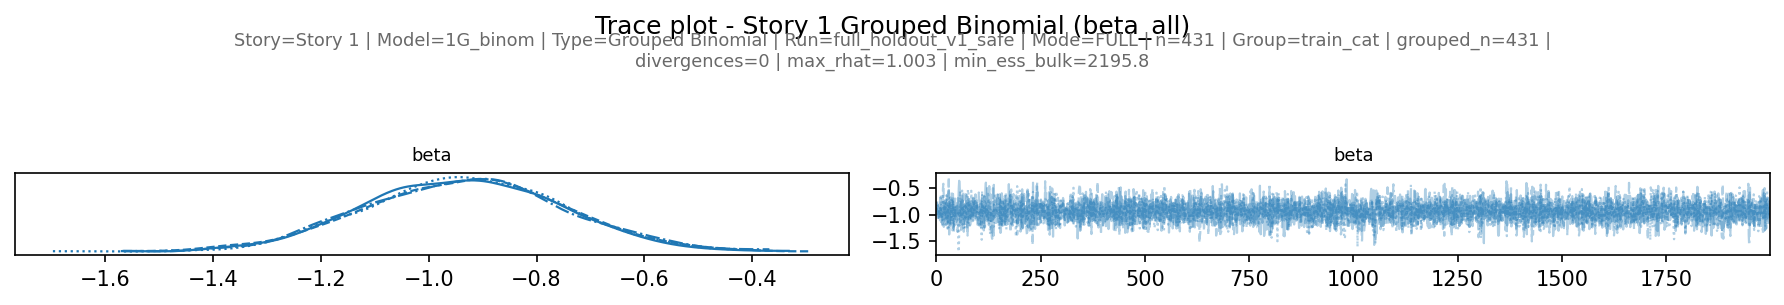
\includegraphics[width=0.8\textwidth]{../../outputs/models/trace_1G_binom_beta_all.png}
    \caption{Trace plot for Story 1 grouped Binomial: \texttt{beta\_all}.}
    \label{fig:trace_1G_beta}
\end{figure}

\begin{figure}[htbp]
    \centering
    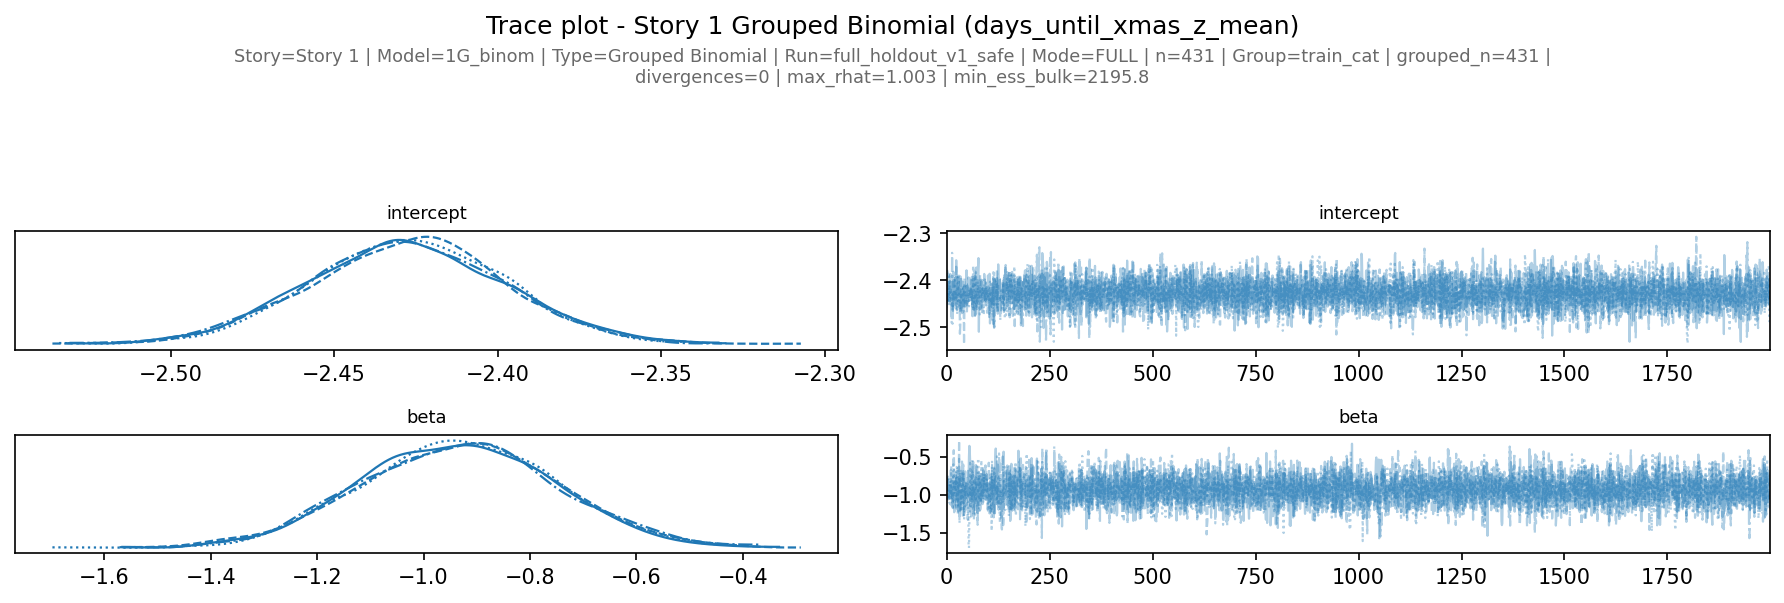
\includegraphics[width=0.8\textwidth]{../../outputs/models/trace_1G_binom_days_until_xmas_z_mean.png}
    \caption{Trace plot for Story 1 grouped Binomial: \texttt{days\_until\_xmas\_z\_mean}.}
    \label{fig:trace_1G_days}
\end{figure}

\FloatBarrier
\clearpage
\subsubsection*{Story 2 incidence models}

\begin{figure}[htbp]
    \centering
    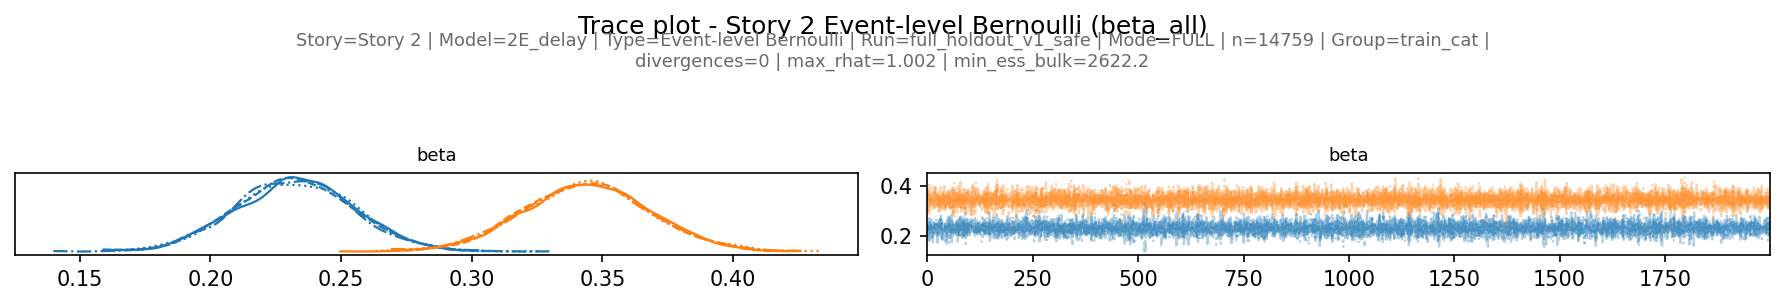
\includegraphics[width=0.8\textwidth]{../../outputs/models/trace_2E_delay_beta_all.png}
    \caption{Trace plot for Story 2 event-level Bernoulli: \texttt{beta\_all}.}
    \label{fig:trace_2E_beta}
\end{figure}

\begin{figure}[htbp]
    \centering
    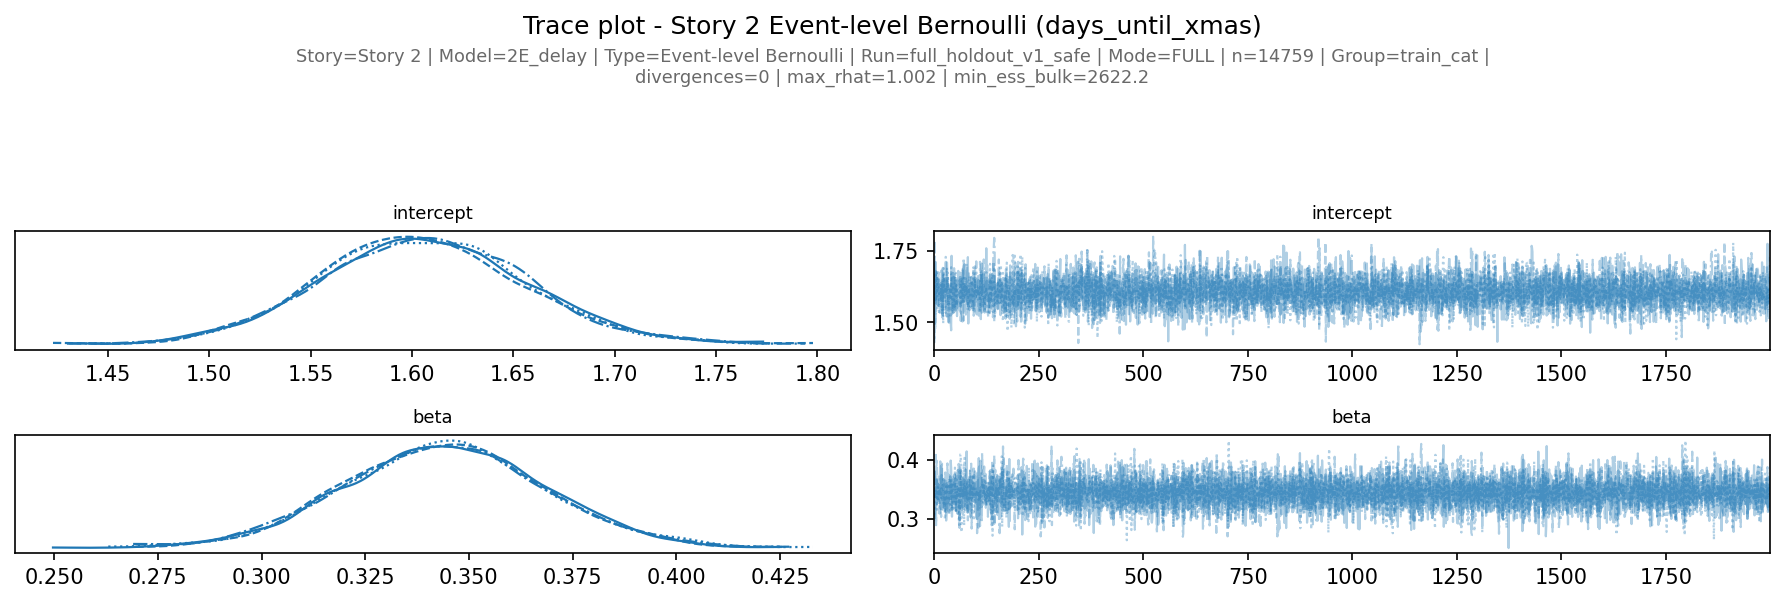
\includegraphics[width=0.8\textwidth]{../../outputs/models/trace_2E_delay_days_until_xmas.png}
    \caption{Trace plot for Story 2 event-level Bernoulli: \texttt{days\_until\_xmas}.}
    \label{fig:trace_2E_days}
\end{figure}

\begin{figure}[htbp]
    \centering
    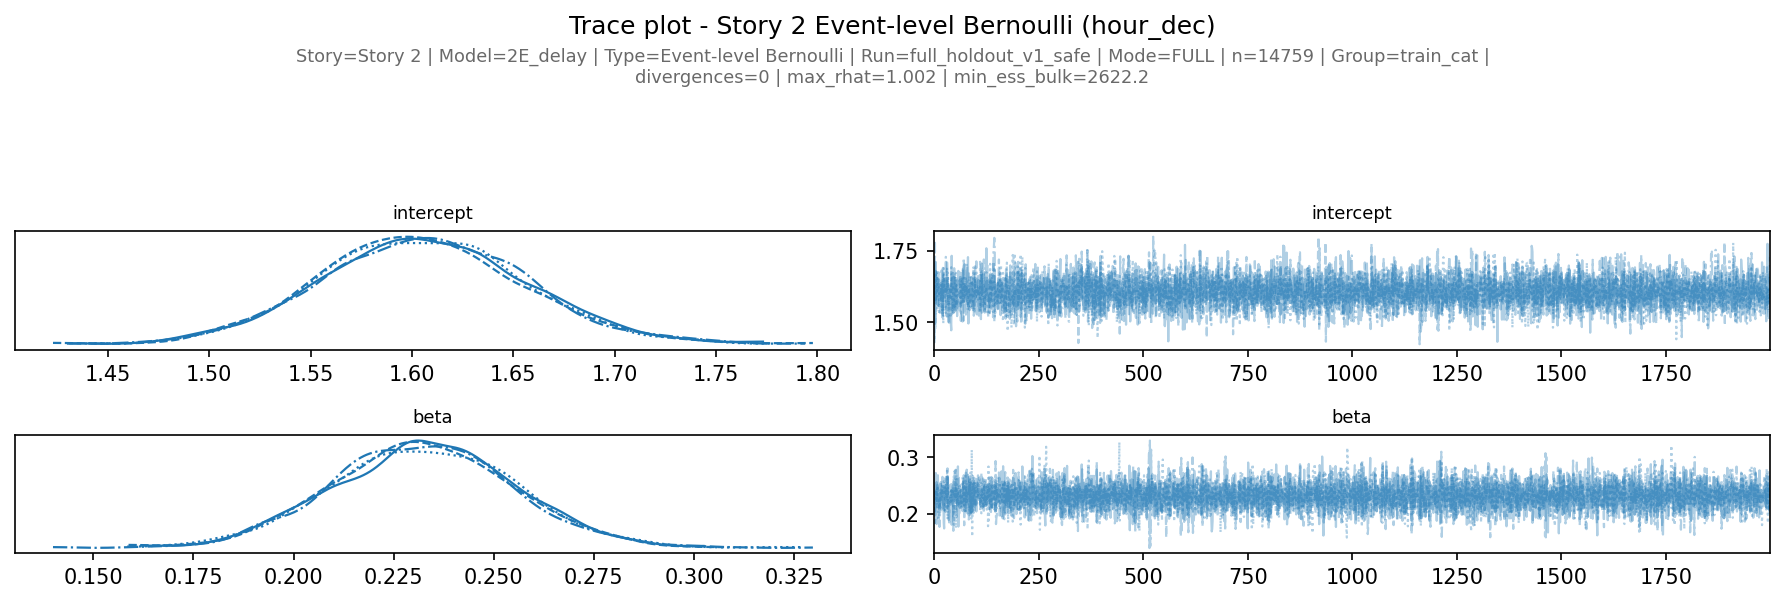
\includegraphics[width=0.8\textwidth]{../../outputs/models/trace_2E_delay_hour_dec.png}
    \caption{Trace plot for Story 2 event-level Bernoulli: \texttt{hour\_dec}.}
    \label{fig:trace_2E_hour}
\end{figure}

\begin{figure}[htbp]
    \centering
    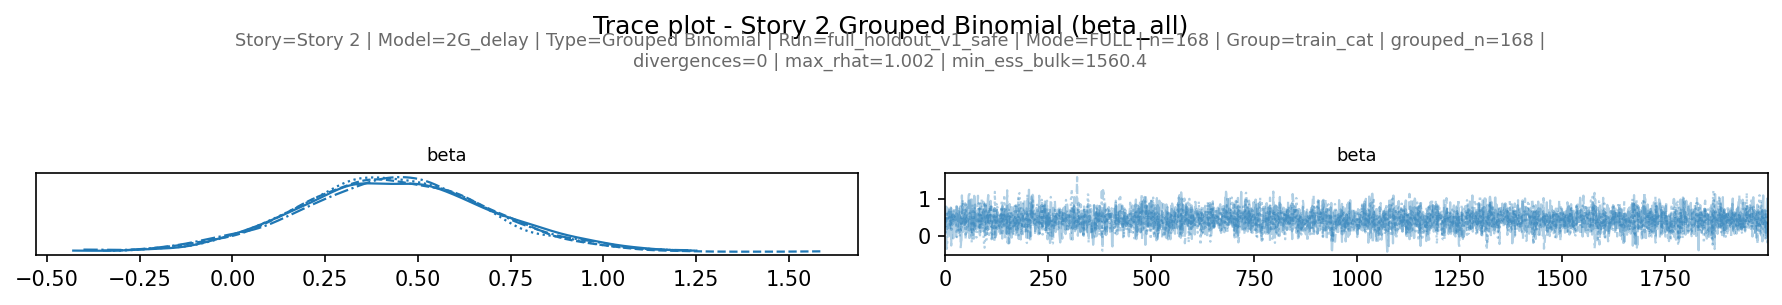
\includegraphics[width=0.8\textwidth]{../../outputs/models/trace_2G_delay_beta_all.png}
    \caption{Trace plot for Story 2 grouped Binomial: \texttt{beta\_all}.}
    \label{fig:trace_2G_beta}
\end{figure}

\begin{figure}[htbp]
    \centering
    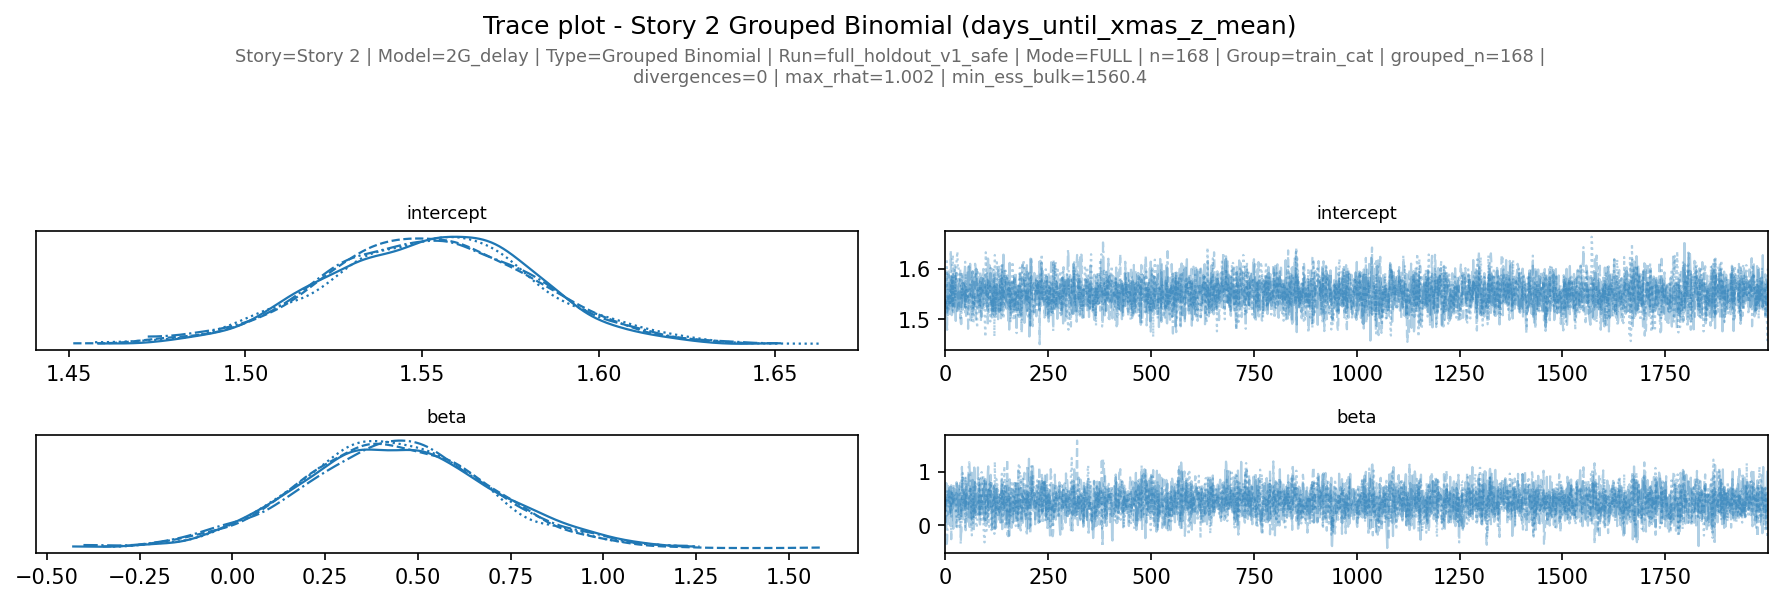
\includegraphics[width=0.8\textwidth]{../../outputs/models/trace_2G_delay_days_until_xmas_z_mean.png}
    \caption{Trace plot for Story 2 grouped Binomial: \texttt{days\_until\_xmas\_z\_mean}.}
    \label{fig:trace_2G_days}
\end{figure}

\FloatBarrier
\clearpage
\subsubsection*{Story 3 incidence models}

\begin{figure}[htbp]
    \centering
    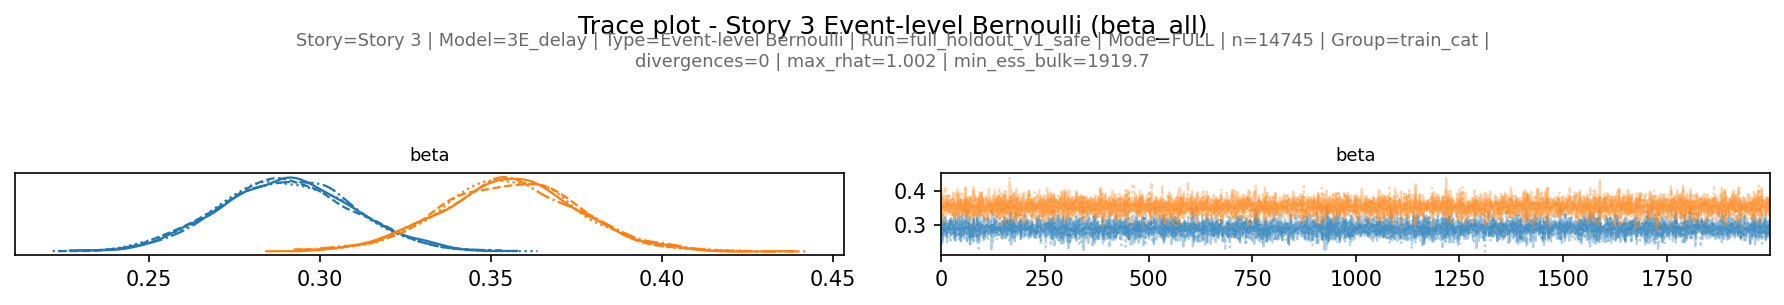
\includegraphics[width=0.8\textwidth]{../../outputs/models/trace_3E_delay_beta_all.png}
    \caption{Trace plot for Story 3 event-level Bernoulli: \texttt{beta\_all}.}
    \label{fig:trace_3E_beta}
\end{figure}

\begin{figure}[htbp]
    \centering
    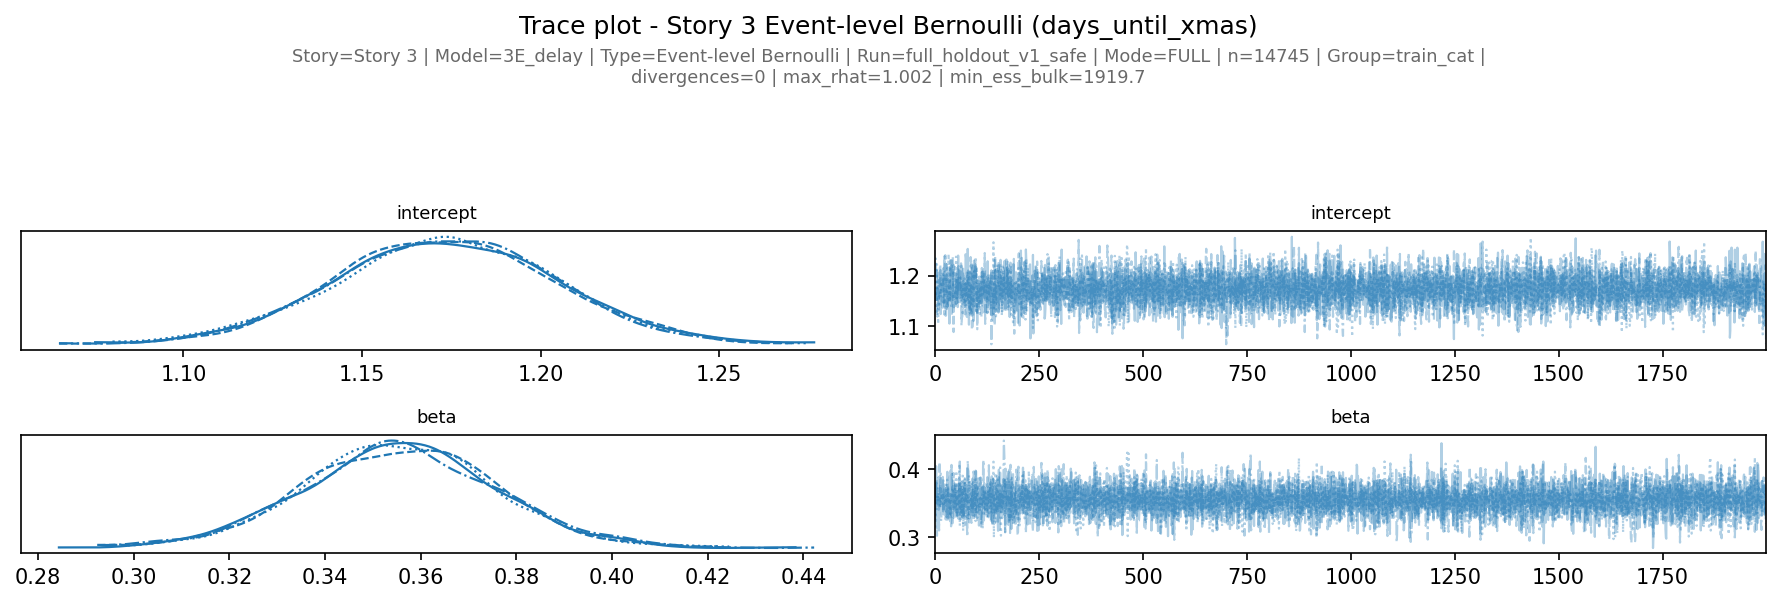
\includegraphics[width=0.8\textwidth]{../../outputs/models/trace_3E_delay_days_until_xmas.png}
    \caption{Trace plot for Story 3 event-level Bernoulli: \texttt{days\_until\_xmas}.}
    \label{fig:trace_3E_days}
\end{figure}

\begin{figure}[htbp]
    \centering
    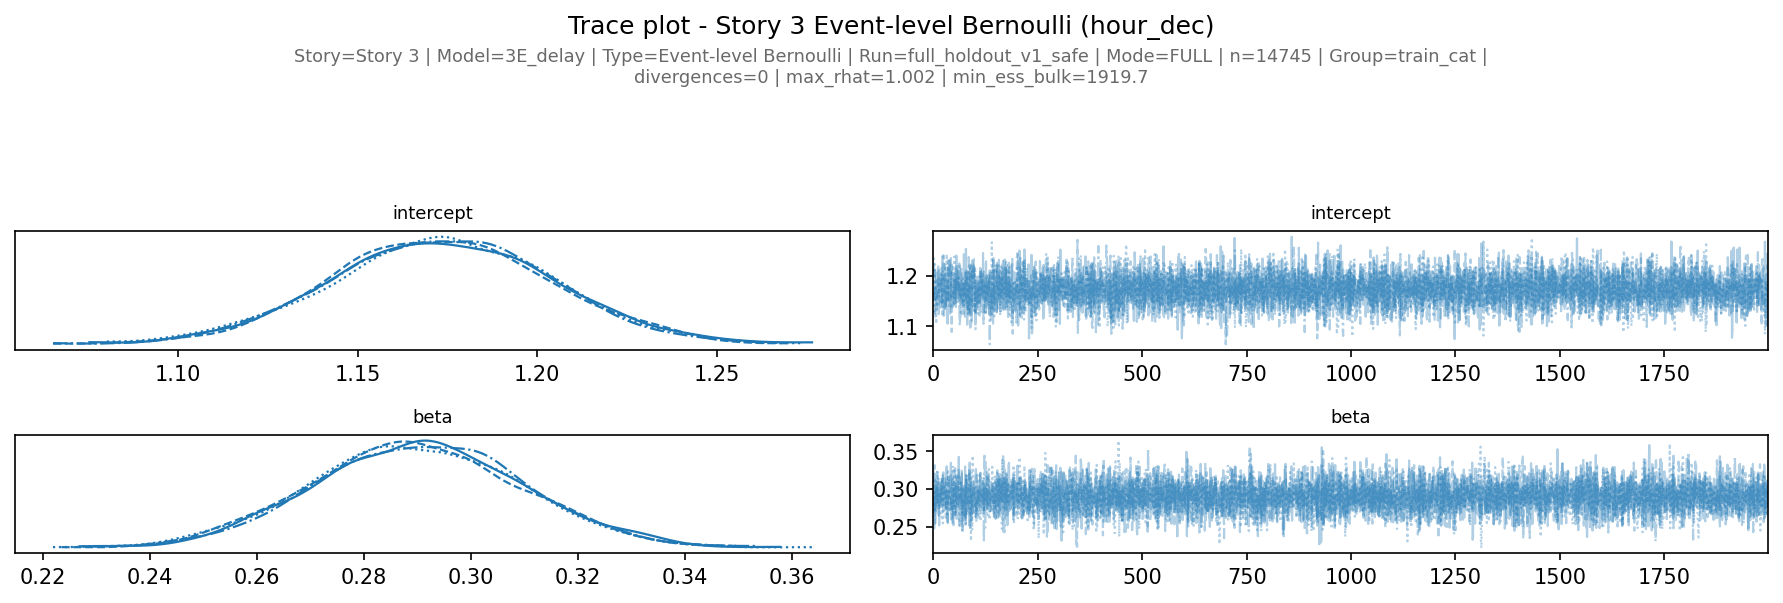
\includegraphics[width=0.8\textwidth]{../../outputs/models/trace_3E_delay_hour_dec.png}
    \caption{Trace plot for Story 3 event-level Bernoulli: \texttt{hour\_dec}.}
    \label{fig:trace_3E_hour}
\end{figure}

\begin{figure}[htbp]
    \centering
    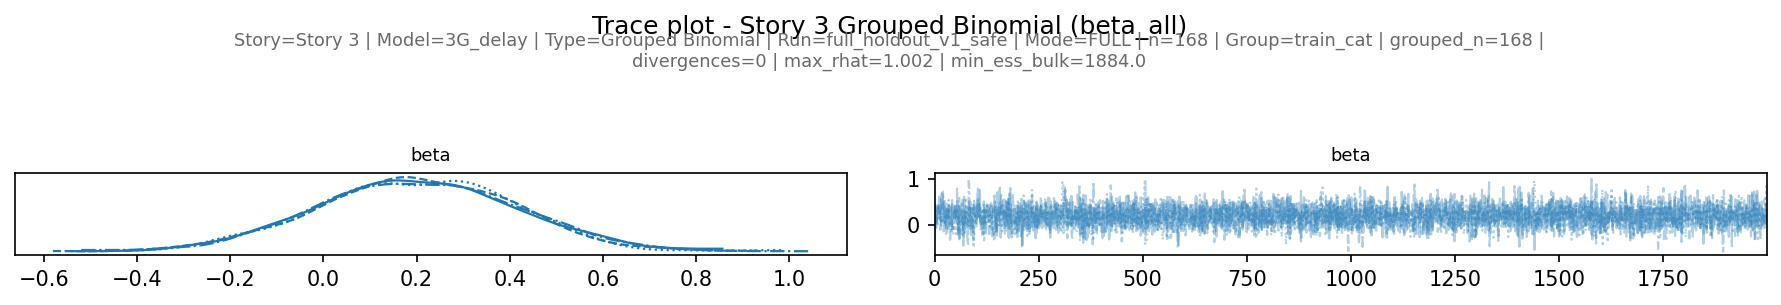
\includegraphics[width=0.8\textwidth]{../../outputs/models/trace_3G_delay_beta_all.png}
    \caption{Trace plot for Story 3 grouped Binomial: \texttt{beta\_all}.}
    \label{fig:trace_3G_beta}
\end{figure}

\begin{figure}[htbp]
    \centering
    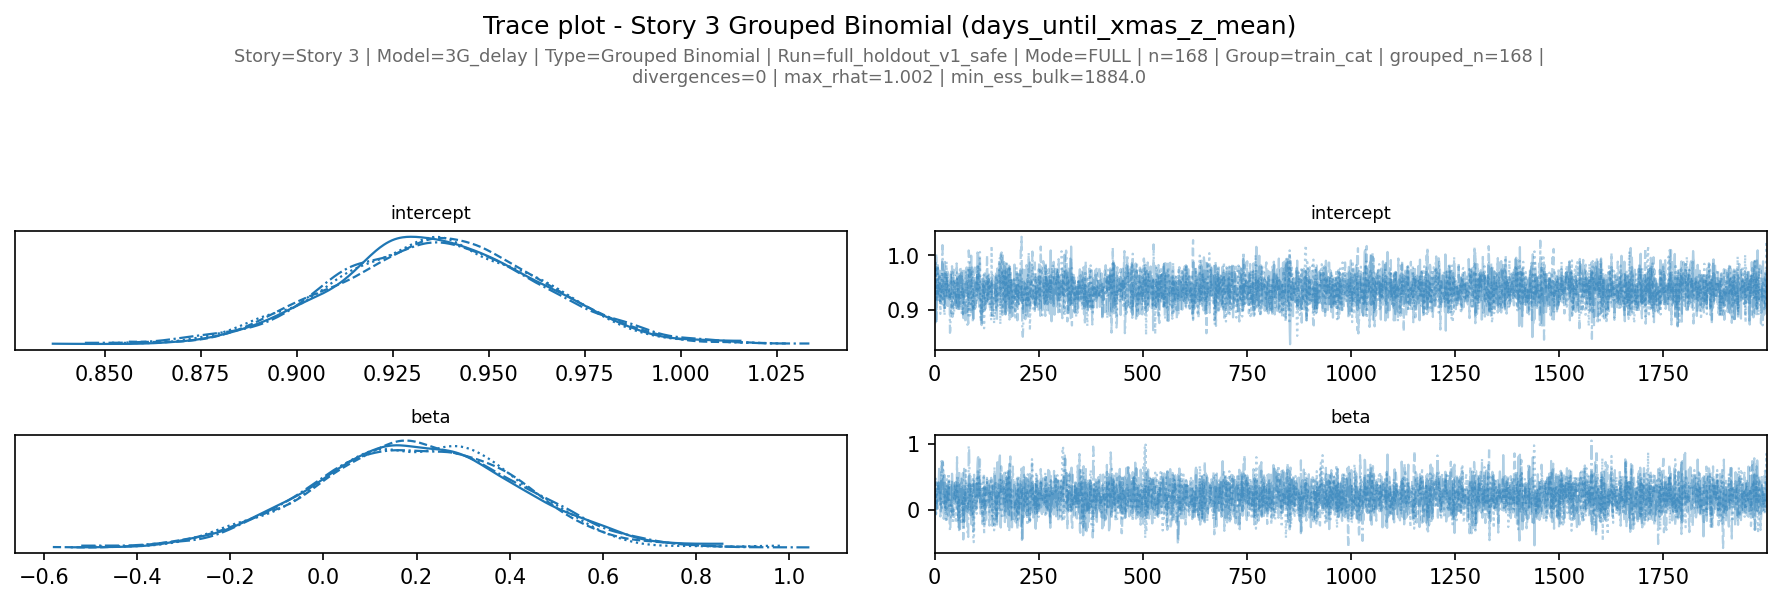
\includegraphics[width=0.8\textwidth]{../../outputs/models/trace_3G_delay_days_until_xmas_z_mean.png}
    \caption{Trace plot for Story 3 grouped Binomial: \texttt{days\_until\_xmas\_z\_mean}.}
    \label{fig:trace_3G_days}
\end{figure}

\FloatBarrier
\clearpage
\subsection{Additional prior predictive checks}
\label{sec:appendix_prior}
\FloatBarrier

\subsubsection*{Story 1}

\begin{figure}[htbp]
    \centering
    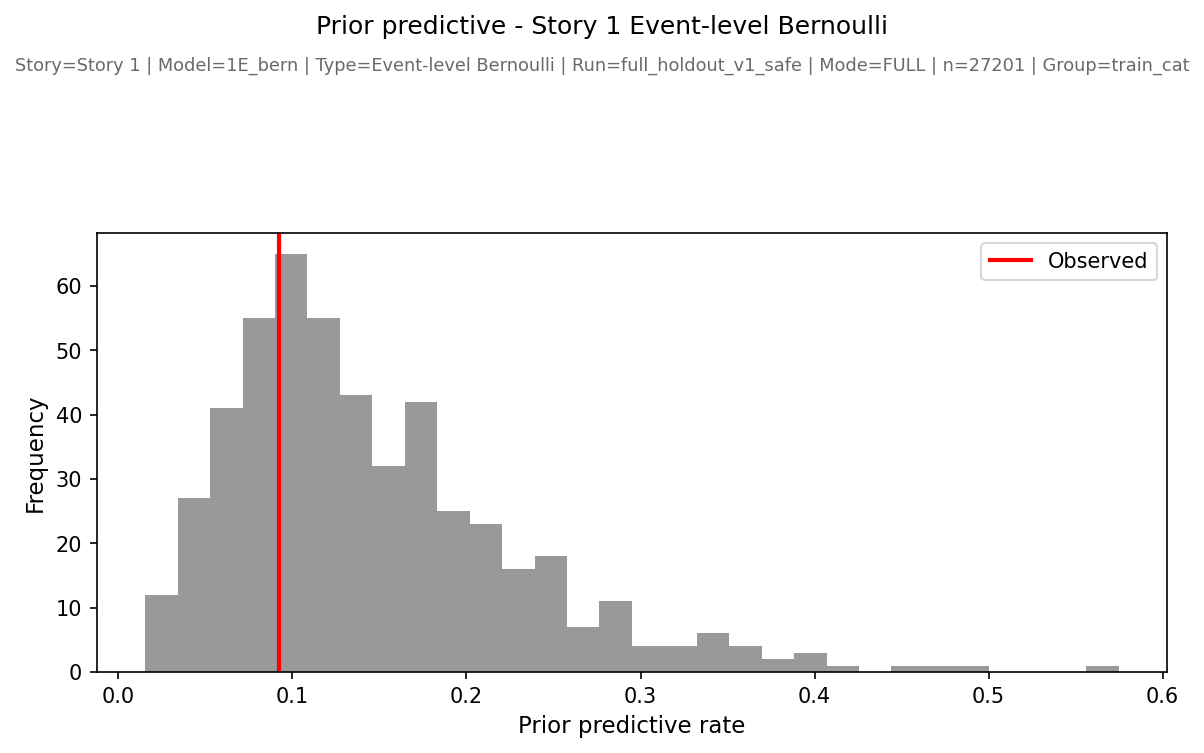
\includegraphics[width=0.72\textwidth]{../../outputs/ppc/prior_1E_bern.png}
    \caption{Prior predictive check for Story 1 event-level Bernoulli.}
    \label{fig:prior_1E_appendix}
\end{figure}

\FloatBarrier
\clearpage
\subsubsection*{Story 2}

\begin{figure}[htbp]
    \centering
    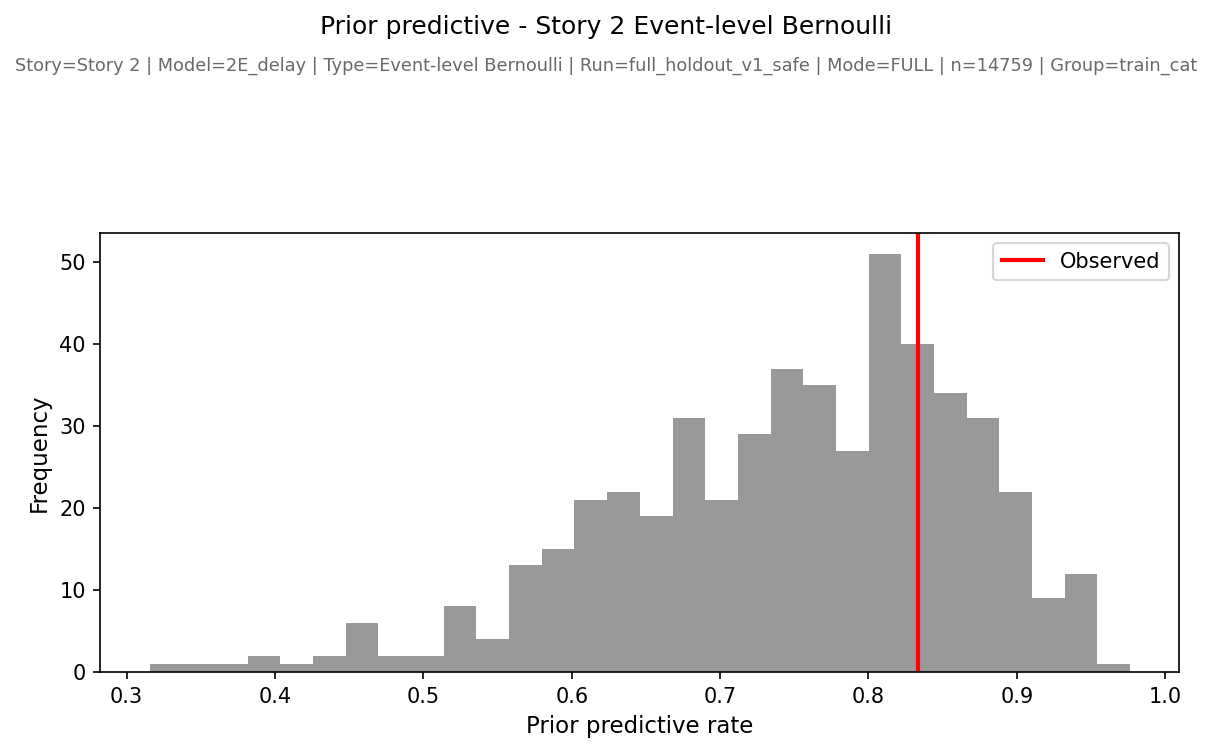
\includegraphics[width=0.72\textwidth]{../../outputs/ppc/prior_2E_delay.png}
    \caption{Prior predictive check for Story 2 event-level Bernoulli.}
    \label{fig:prior_2E_appendix}
\end{figure}

\FloatBarrier
\clearpage
\subsubsection*{Story 3}

\begin{figure}[htbp]
    \centering
    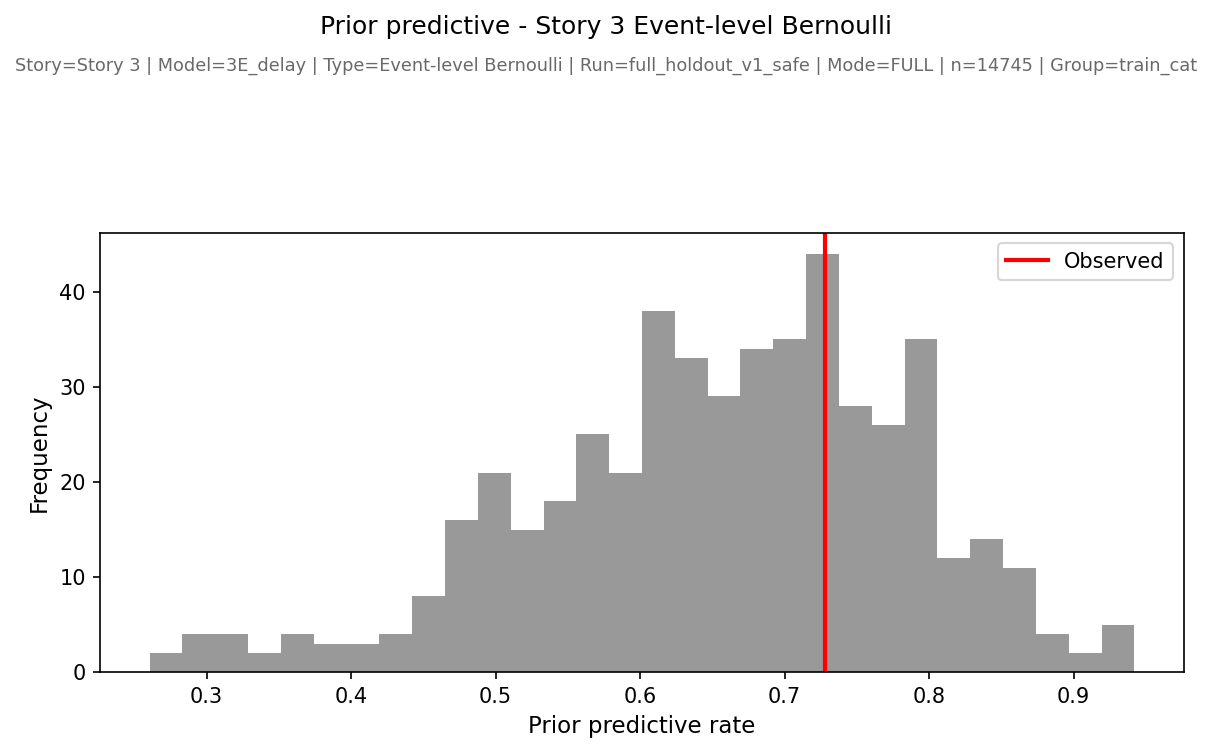
\includegraphics[width=0.72\textwidth]{../../outputs/ppc/prior_3E_delay.png}
    \caption{Prior predictive check for Story 3 event-level Bernoulli.}
    \label{fig:prior_3E_appendix}
\end{figure}

\FloatBarrier
\clearpage
\subsection{Additional posterior predictive checks}
\label{sec:appendix_ppc}
\FloatBarrier

\subsubsection*{Story 1}

\begin{figure}[htbp]
    \centering
    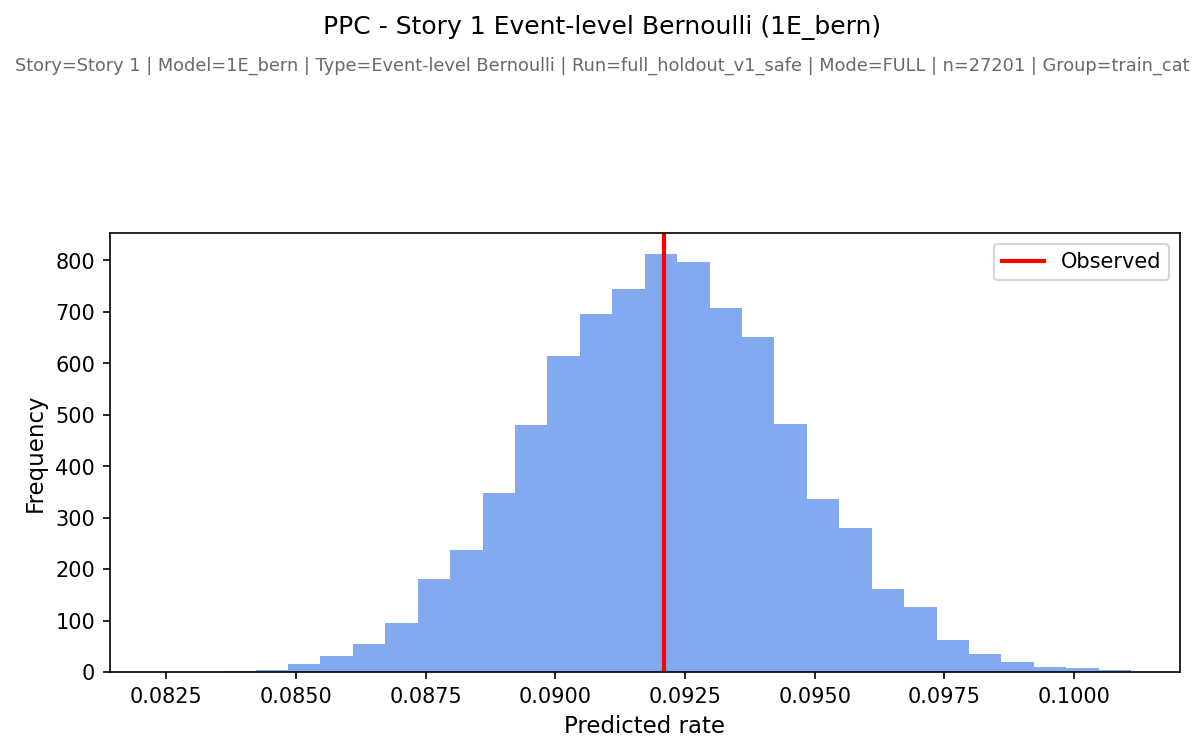
\includegraphics[width=0.72\textwidth]{../../outputs/ppc/ppc_1E_bern.png}
    \caption{Posterior predictive check for Story 1 event-level Bernoulli.}
    \label{fig:ppc_1E_appendix}
\end{figure}

\begin{figure}[htbp]
    \centering
    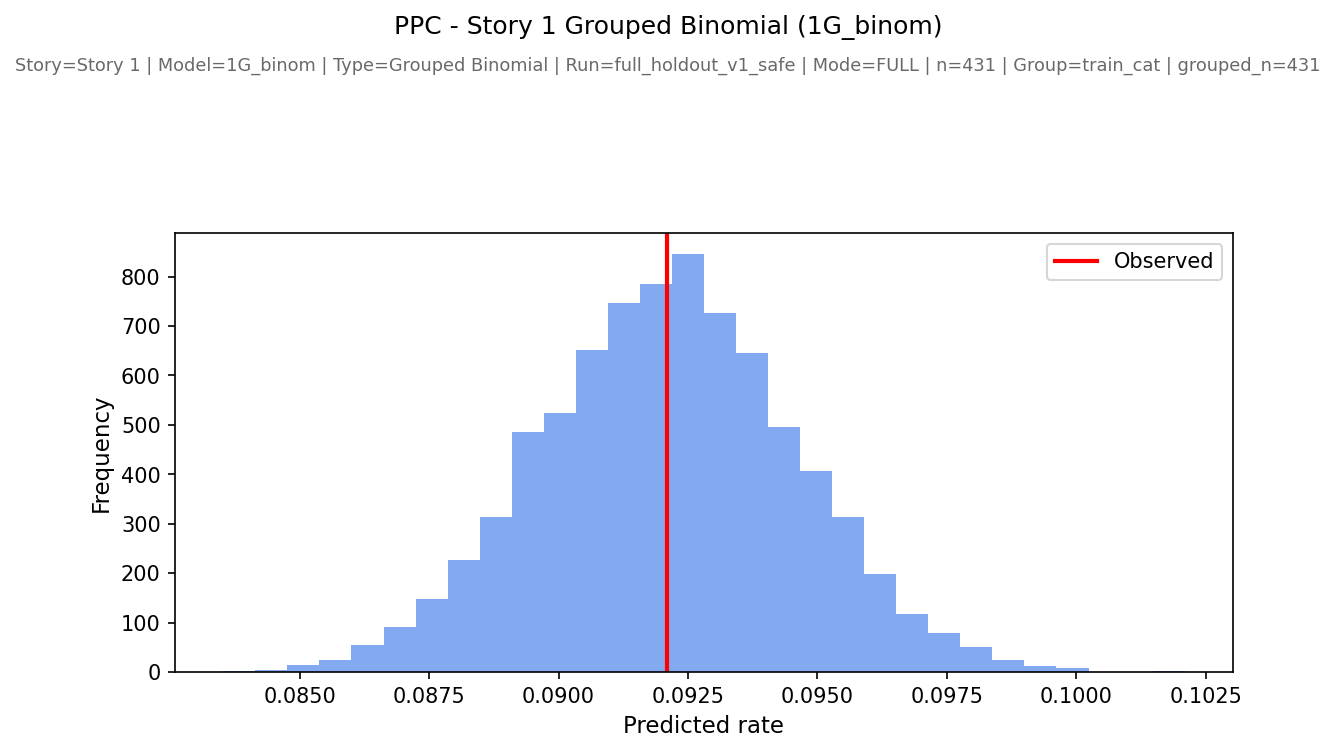
\includegraphics[width=0.72\textwidth]{../../outputs/ppc/ppc_1G_binom.png}
    \caption{Posterior predictive check for Story 1 grouped Binomial.}
    \label{fig:ppc_1G_appendix}
\end{figure}

\FloatBarrier
\clearpage
\subsubsection*{Story 2}

\begin{figure}[htbp]
    \centering
    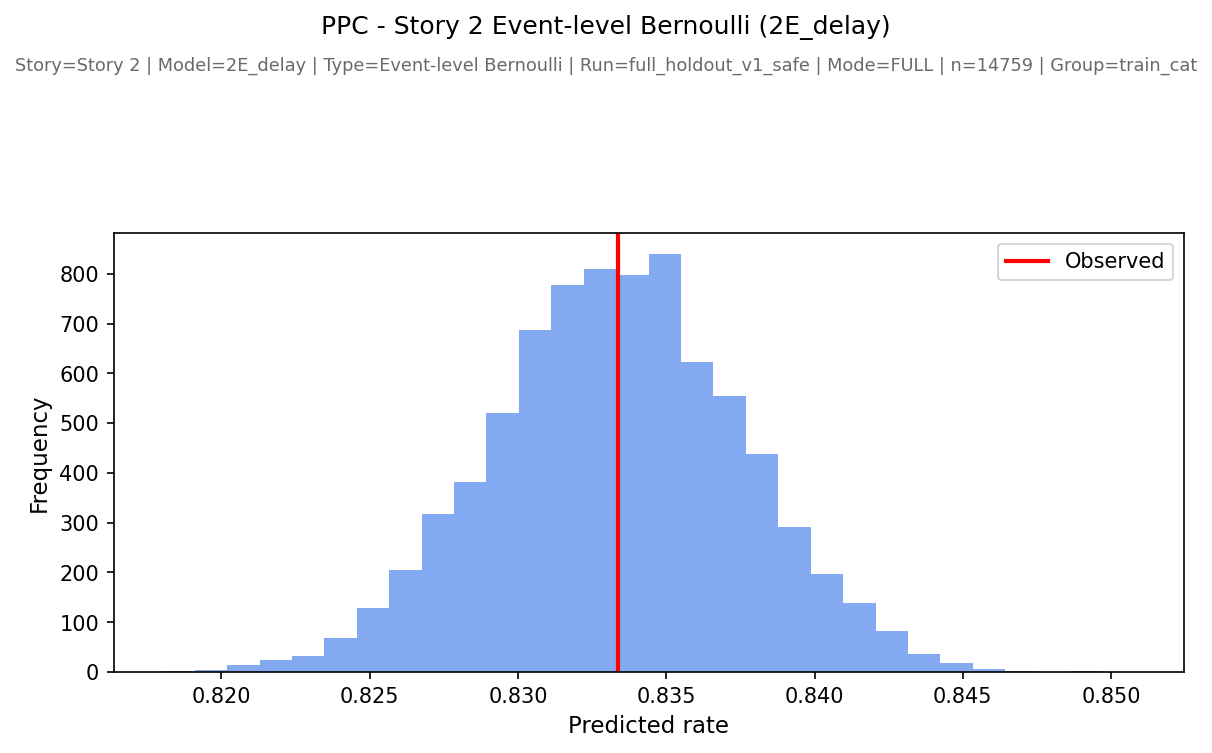
\includegraphics[width=0.72\textwidth]{../../outputs/ppc/ppc_2E_delay.png}
    \caption{Posterior predictive check for Story 2 event-level Bernoulli.}
    \label{fig:ppc_2E_appendix}
\end{figure}

\begin{figure}[htbp]
    \centering
    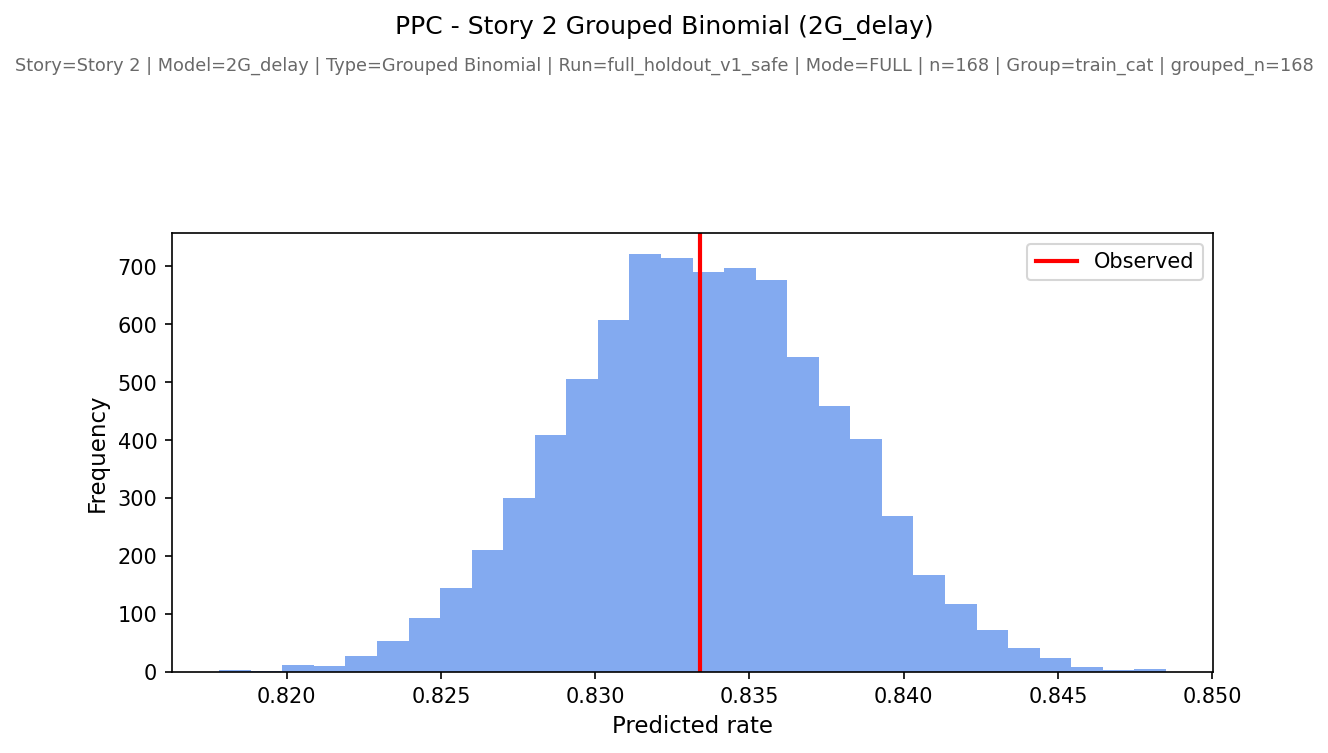
\includegraphics[width=0.72\textwidth]{../../outputs/ppc/ppc_2G_delay.png}
    \caption{Posterior predictive check for Story 2 grouped Binomial.}
    \label{fig:ppc_2G_appendix}
\end{figure}

\begin{figure}[htbp]
    \centering
    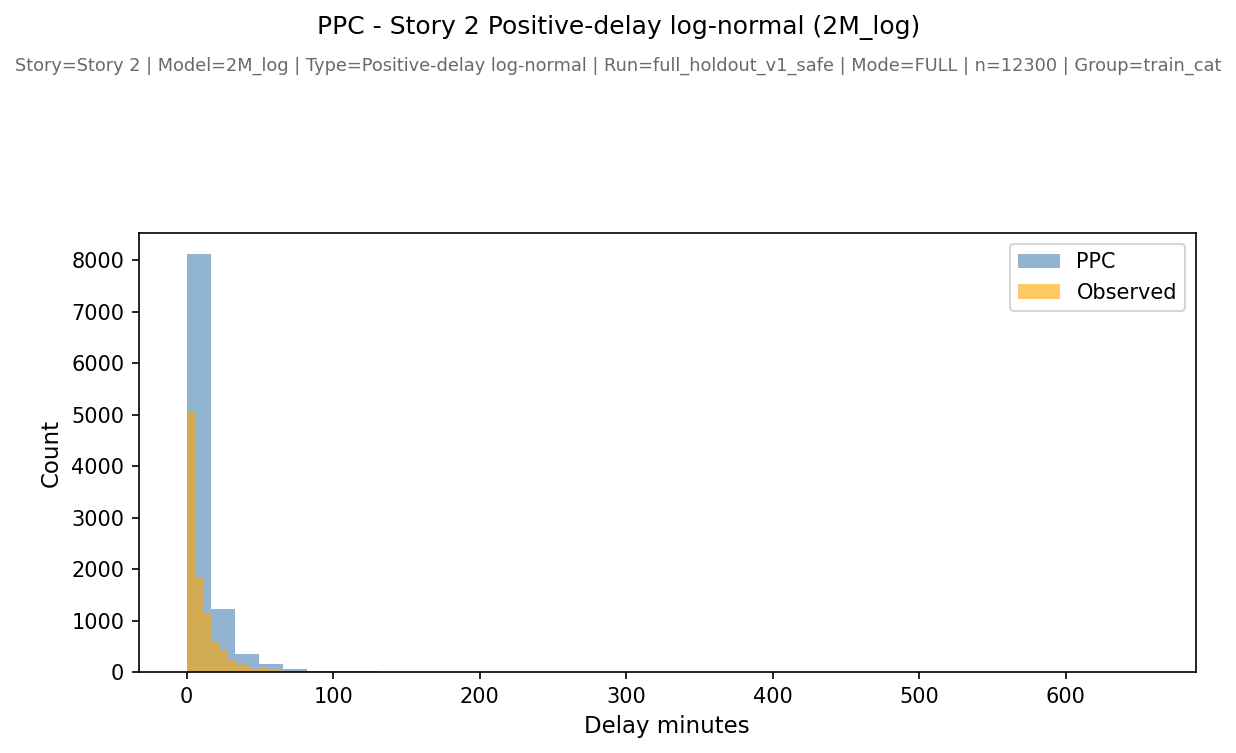
\includegraphics[width=0.72\textwidth]{../../outputs/ppc/ppc_2M_log.png}
    \caption{Posterior predictive check for Story 2 positive-delay log-normal support model.}
    \label{fig:ppc_2M_appendix}
\end{figure}

\FloatBarrier
\clearpage
\subsubsection*{Story 3}

\begin{figure}[htbp]
    \centering
    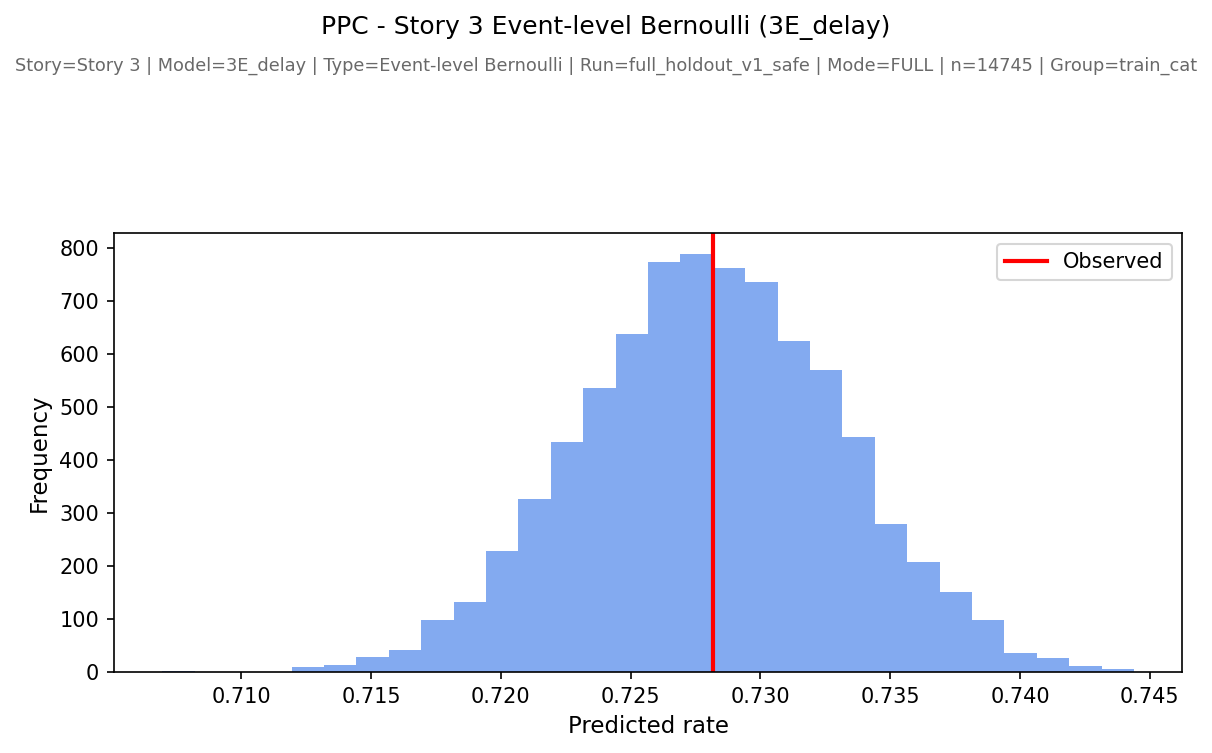
\includegraphics[width=0.72\textwidth]{../../outputs/ppc/ppc_3E_delay.png}
    \caption{Posterior predictive check for Story 3 event-level Bernoulli.}
    \label{fig:ppc_3E_appendix}
\end{figure}

\begin{figure}[htbp]
    \centering
    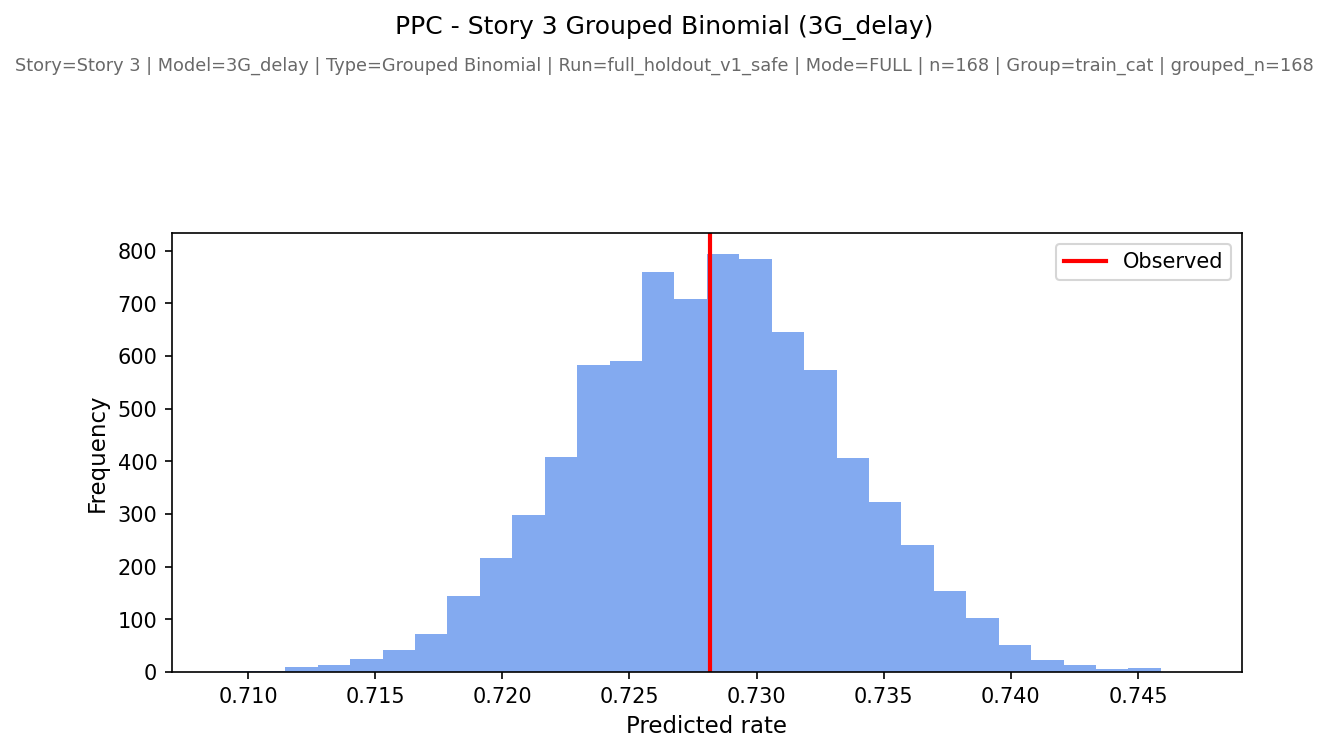
\includegraphics[width=0.72\textwidth]{../../outputs/ppc/ppc_3G_delay.png}
    \caption{Posterior predictive check for Story 3 grouped Binomial.}
    \label{fig:ppc_3G_appendix}
\end{figure}

\begin{figure}[htbp]
    \centering
    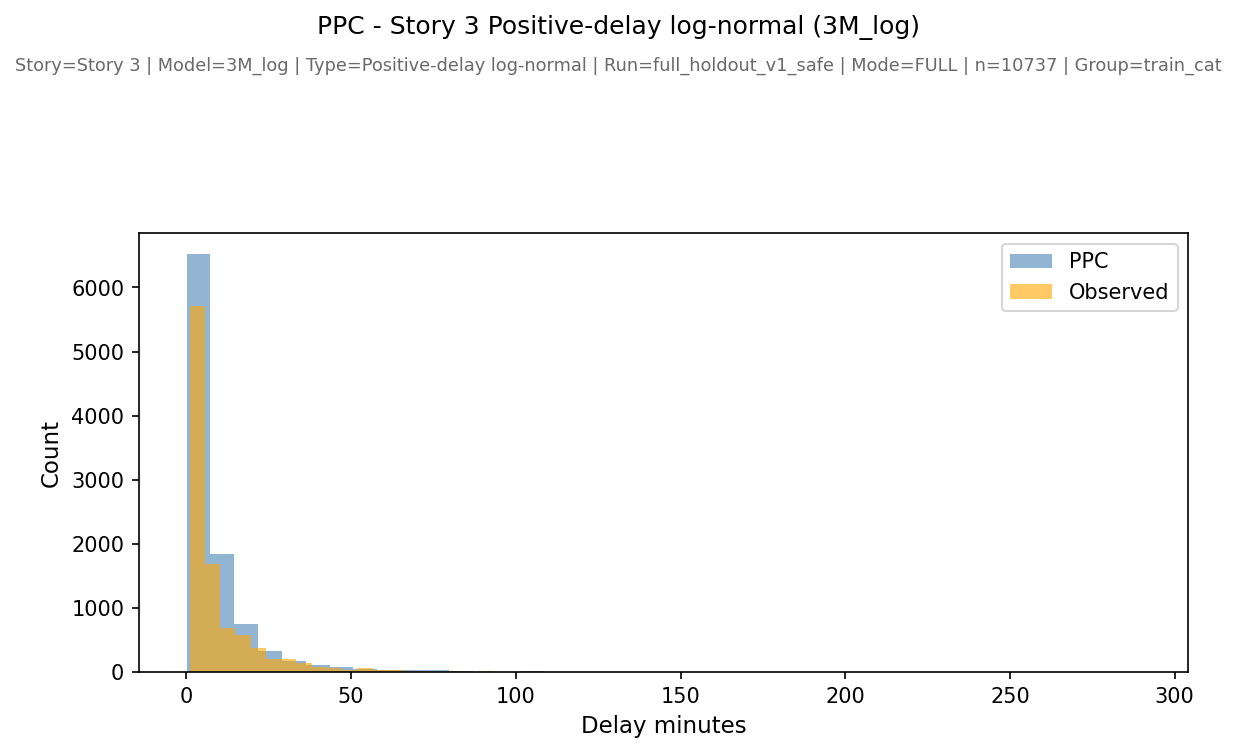
\includegraphics[width=0.72\textwidth]{../../outputs/ppc/ppc_3M_log.png}
    \caption{Posterior predictive check for Story 3 positive-delay log-normal support model.}
    \label{fig:ppc_3M_appendix}
\end{figure}

\FloatBarrier
\clearpage
\subsection{Additional calibration and exchangeability figures}
\label{sec:appendix_calibration}
\label{sec:appendix_checks}
\FloatBarrier

The following figures report story-specific calibration, posterior \texttt{train\_cat} effects, posterior category probabilities, and observed-rate versus reference-scenario probability comparisons for the Phase~2 incidence models.

\subsubsection*{Story 1}

\begin{figure}[htbp]
    \centering
    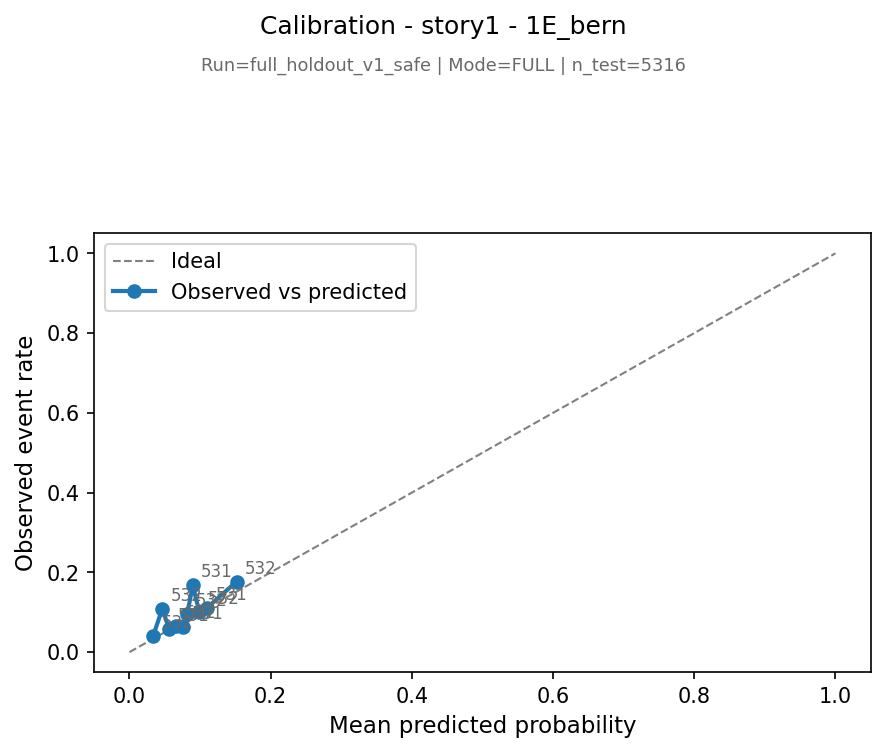
\includegraphics[width=0.72\textwidth]{../../outputs/ppc/story1_calibration_1E_bern.png}
    \caption{Calibration for Story 1 event-level Bernoulli.}
    \label{fig:story1_calib_1E_appendix}
\end{figure}

\begin{figure}[htbp]
    \centering
    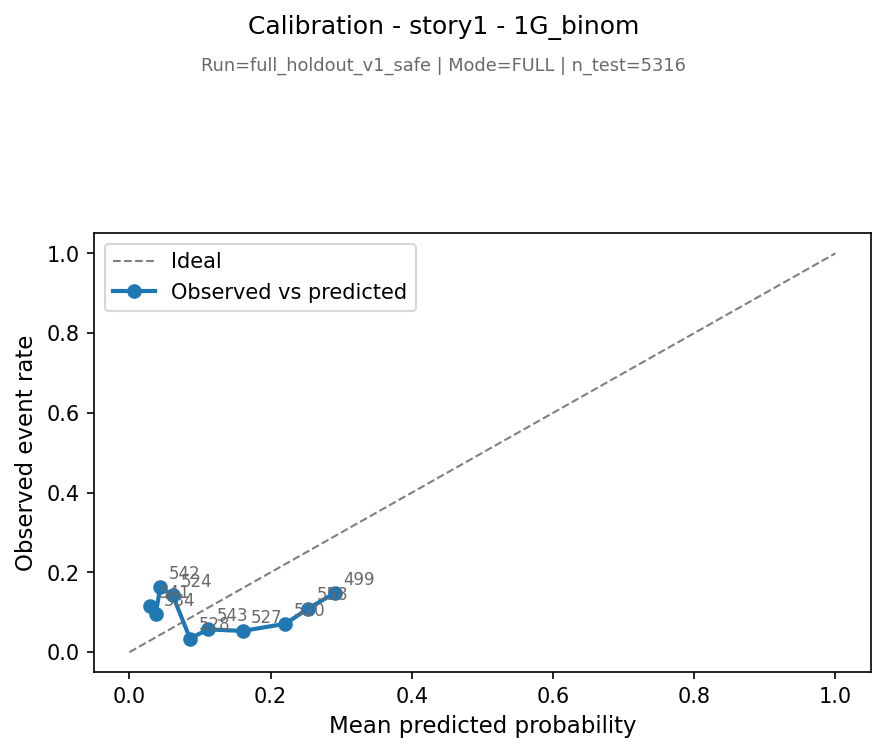
\includegraphics[width=0.72\textwidth]{../../outputs/ppc/story1_calibration_1G_binom.png}
    \caption{Calibration for Story 1 grouped Binomial.}
    \label{fig:story1_calib_1G_appendix}
\end{figure}

\begin{figure}[htbp]
    \centering
    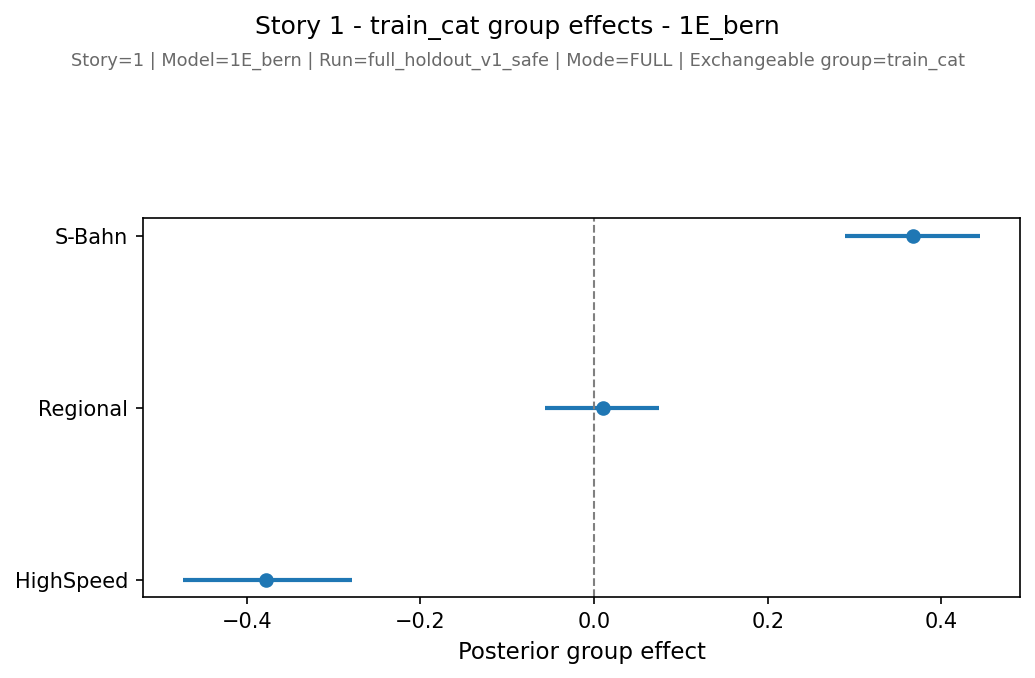
\includegraphics[width=0.72\textwidth]{../../outputs/ppc/story1_train_cat_effects_1E_bern.png}
    \caption{\texttt{train\_cat} effects for Story 1 event-level Bernoulli.}
    \label{fig:story1_eff_1E_appendix}
\end{figure}

\begin{figure}[htbp]
    \centering
    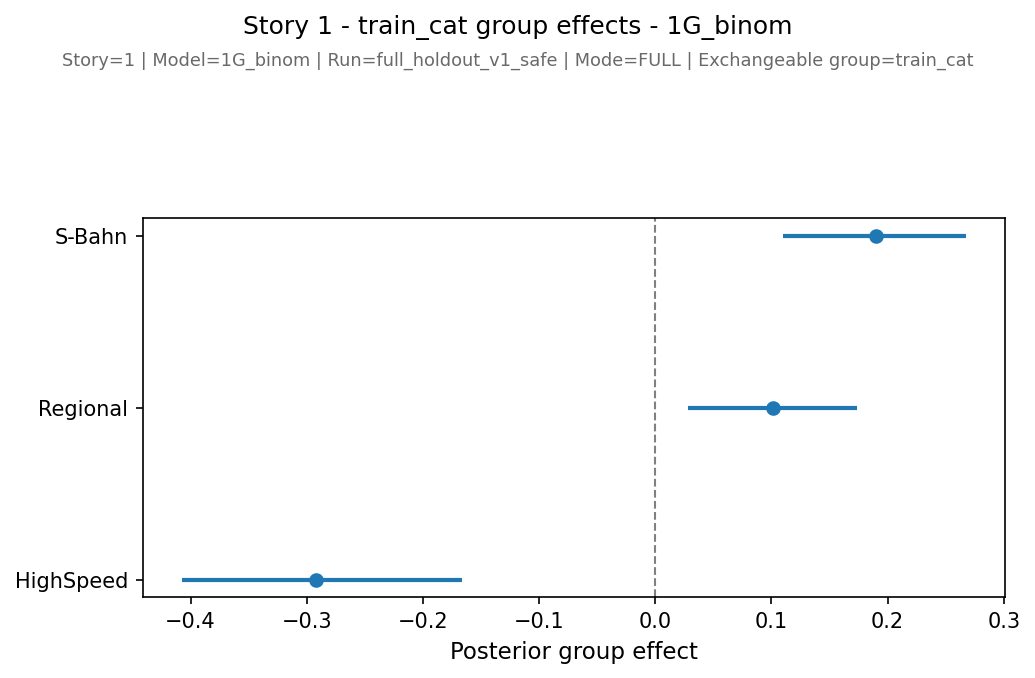
\includegraphics[width=0.72\textwidth]{../../outputs/ppc/story1_train_cat_effects_1G_binom.png}
    \caption{\texttt{train\_cat} effects for Story 1 grouped Binomial.}
    \label{fig:story1_eff_1G_appendix}
\end{figure}

\begin{figure}[htbp]
    \centering
    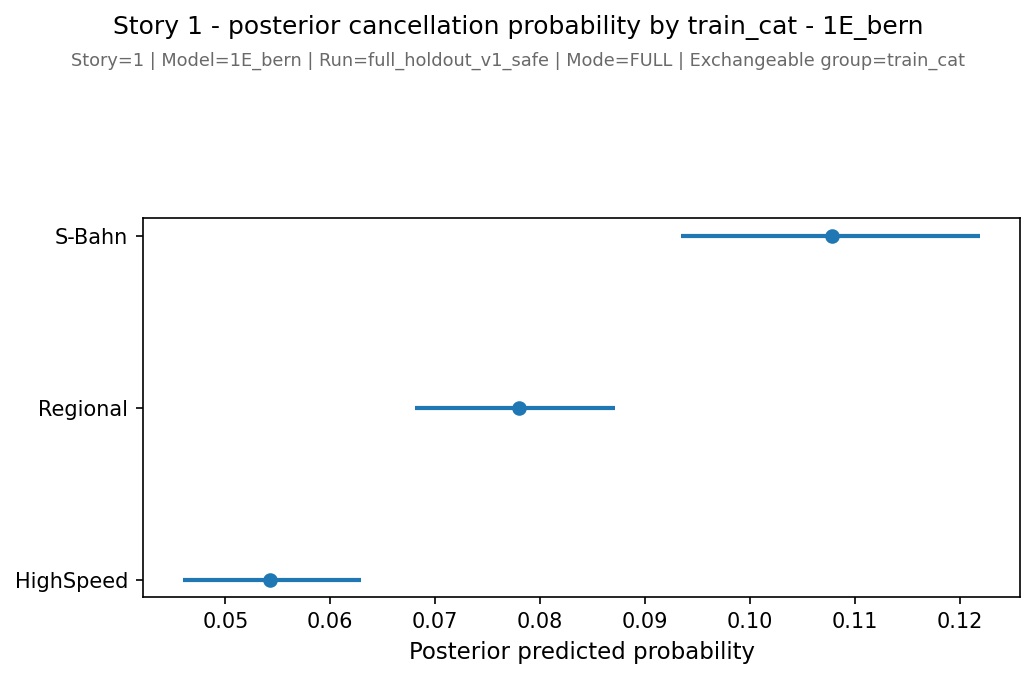
\includegraphics[width=0.72\textwidth]{../../outputs/ppc/story1_train_cat_probs_1E_bern.png}
    \caption{Posterior \texttt{train\_cat} probabilities for Story 1 event-level Bernoulli.}
    \label{fig:story1_prob_1E_appendix}
\end{figure}

\begin{figure}[htbp]
    \centering
    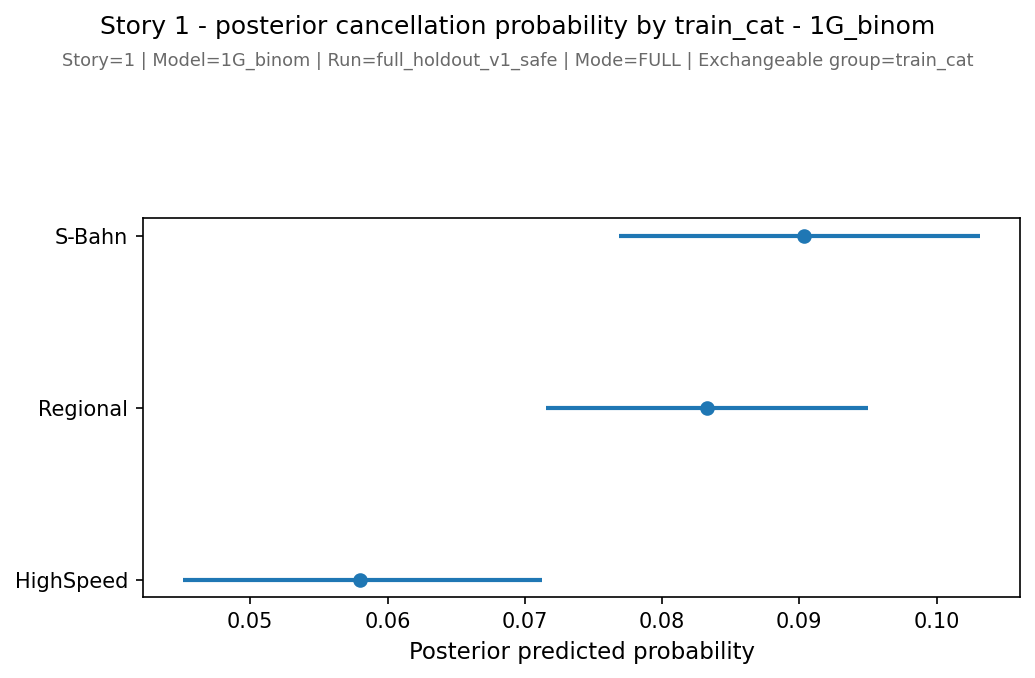
\includegraphics[width=0.72\textwidth]{../../outputs/ppc/story1_train_cat_probs_1G_binom.png}
    \caption{Posterior \texttt{train\_cat} probabilities for Story 1 grouped Binomial.}
    \label{fig:story1_prob_1G_appendix}
\end{figure}

\begin{figure}[htbp]
    \centering
    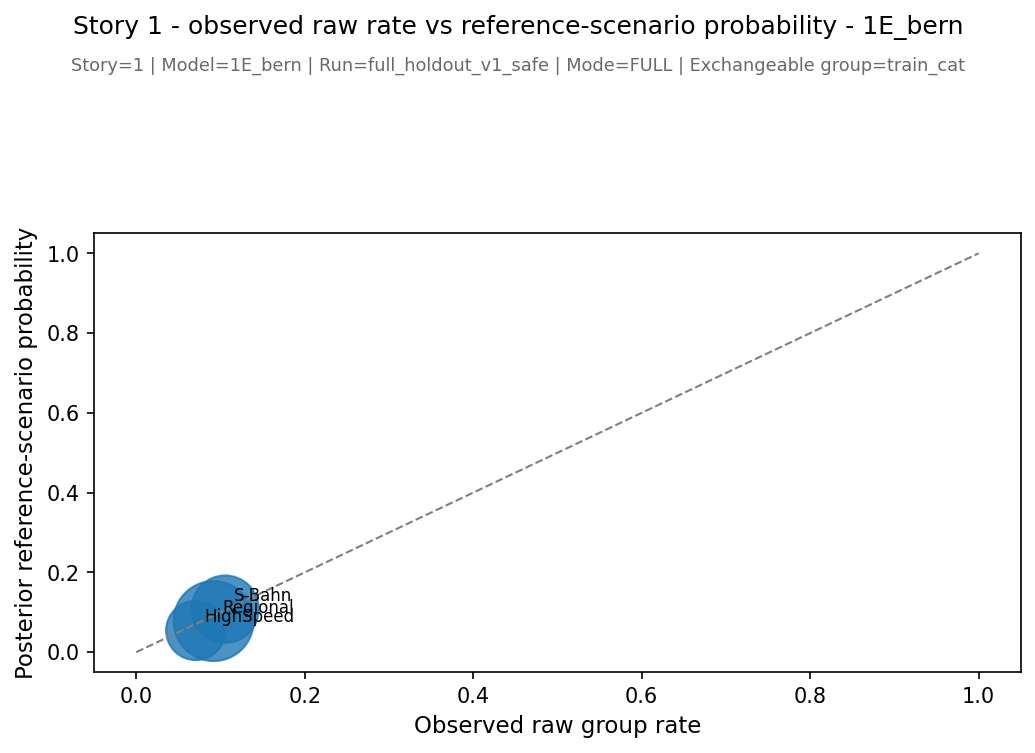
\includegraphics[width=0.72\textwidth]{../../outputs/ppc/story1_obs_vs_refprob_1E_bern.png}
    \caption{Observed raw rates versus reference-scenario posterior probabilities for Story 1 event-level Bernoulli.}
    \label{fig:story1_ref_1E_appendix}
\end{figure}

\begin{figure}[htbp]
    \centering
    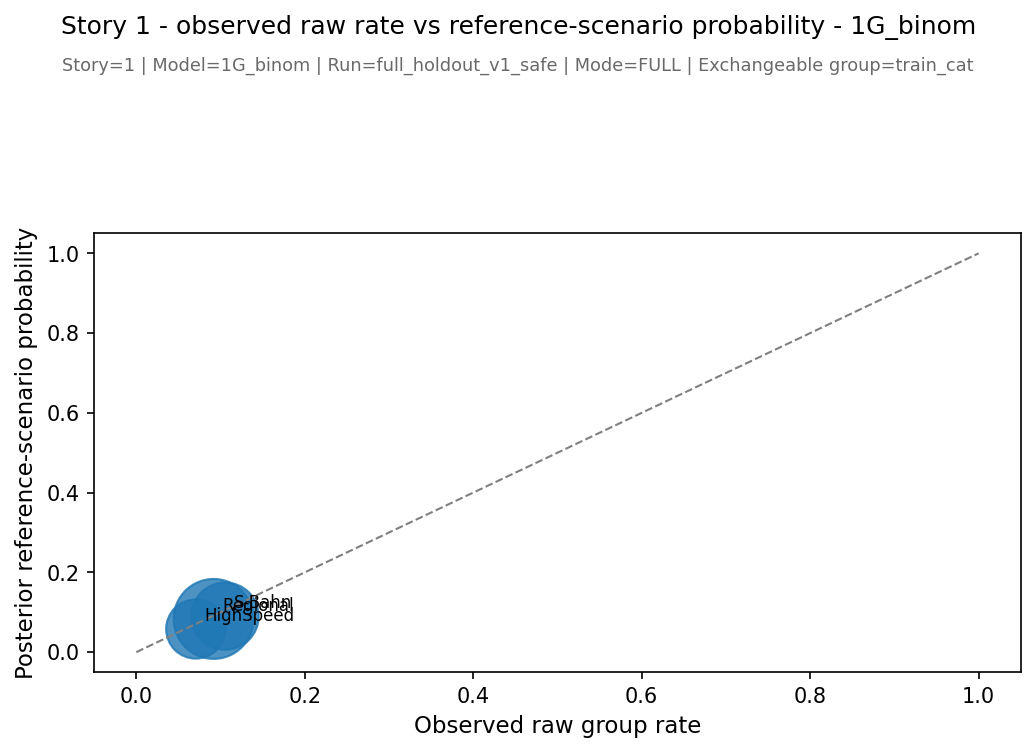
\includegraphics[width=0.72\textwidth]{../../outputs/ppc/story1_obs_vs_refprob_1G_binom.png}
    \caption{Observed raw rates versus reference-scenario posterior probabilities for Story 1 grouped Binomial.}
    \label{fig:story1_ref_1G_appendix}
\end{figure}

\FloatBarrier
\clearpage
\subsubsection*{Story 2}

\begin{figure}[htbp]
    \centering
    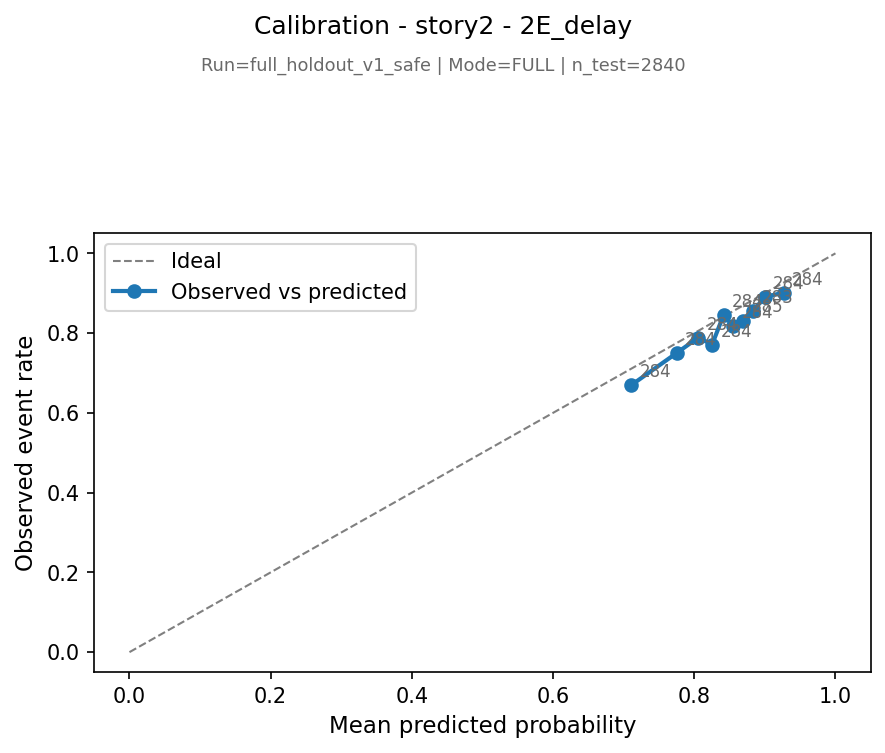
\includegraphics[width=0.72\textwidth]{../../outputs/ppc/story2_calibration_2E_delay.png}
    \caption{Calibration for Story 2 event-level Bernoulli.}
    \label{fig:story2_calib_2E_appendix}
\end{figure}

\begin{figure}[htbp]
    \centering
    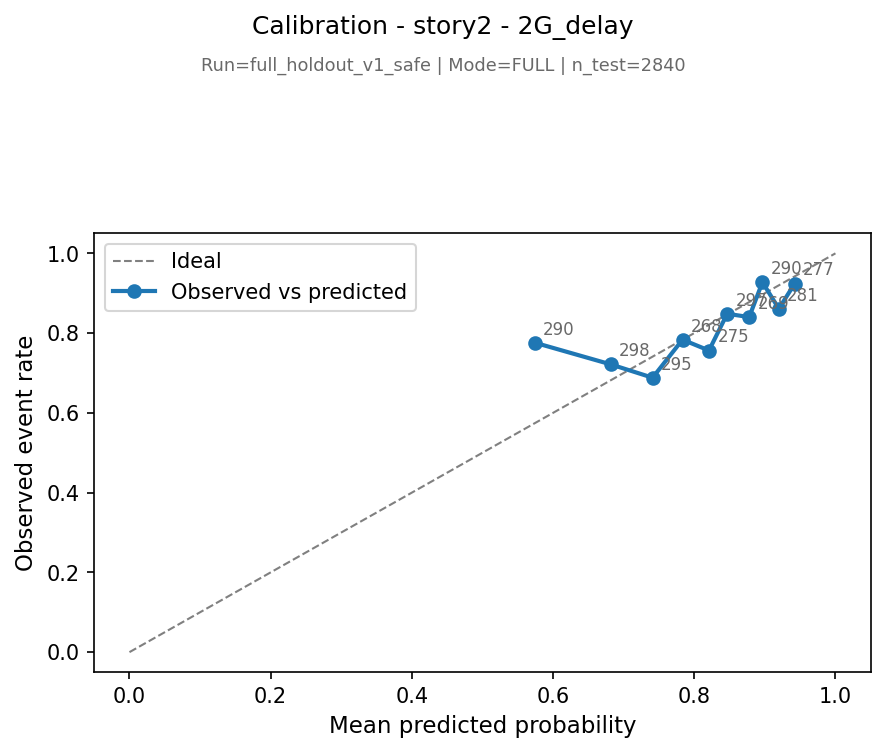
\includegraphics[width=0.72\textwidth]{../../outputs/ppc/story2_calibration_2G_delay.png}
    \caption{Calibration for Story 2 grouped Binomial.}
    \label{fig:story2_calib_2G_appendix}
\end{figure}

\begin{figure}[htbp]
    \centering
    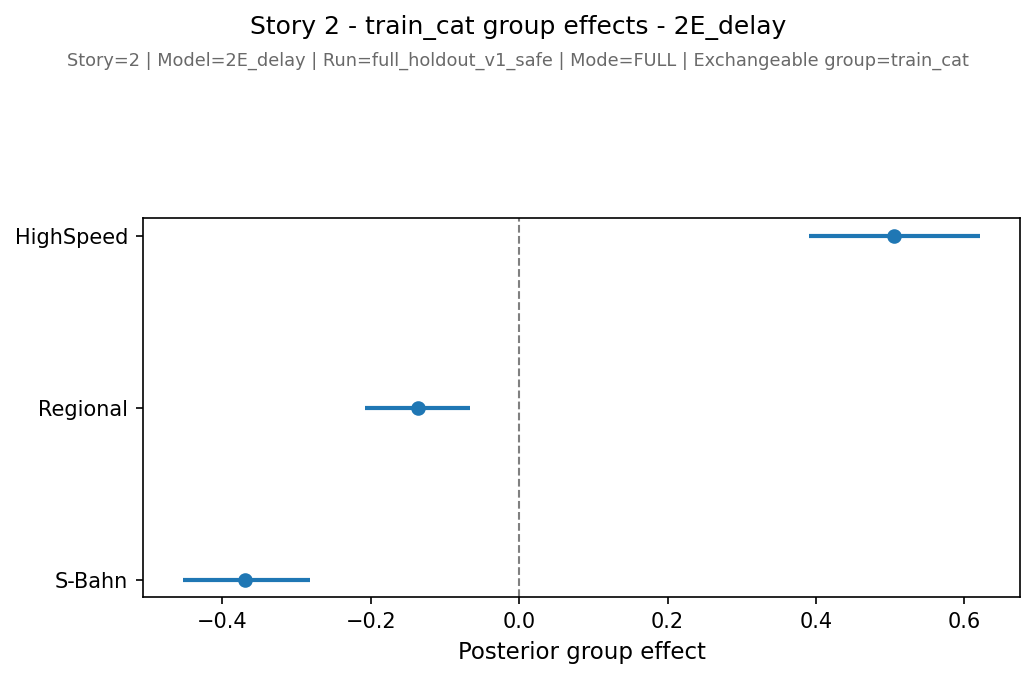
\includegraphics[width=0.72\textwidth]{../../outputs/ppc/story2_train_cat_effects_2E_delay.png}
    \caption{\texttt{train\_cat} effects for Story 2 event-level Bernoulli.}
    \label{fig:story2_eff_2E_appendix}
\end{figure}

\begin{figure}[htbp]
    \centering
    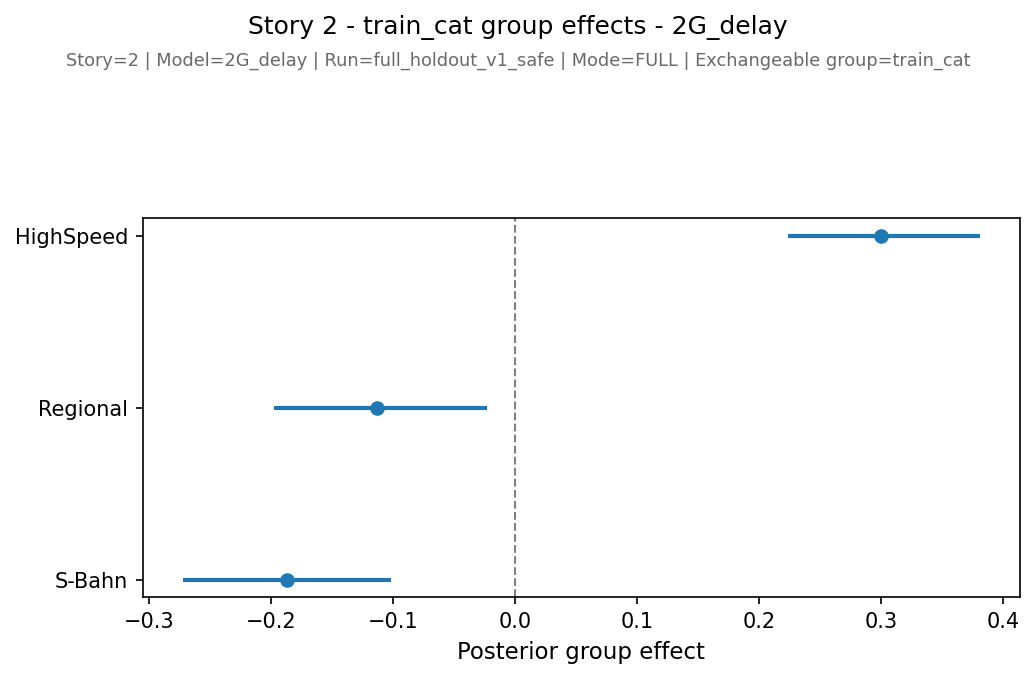
\includegraphics[width=0.72\textwidth]{../../outputs/ppc/story2_train_cat_effects_2G_delay.png}
    \caption{\texttt{train\_cat} effects for Story 2 grouped Binomial.}
    \label{fig:story2_eff_2G_appendix}
\end{figure}

\begin{figure}[htbp]
    \centering
    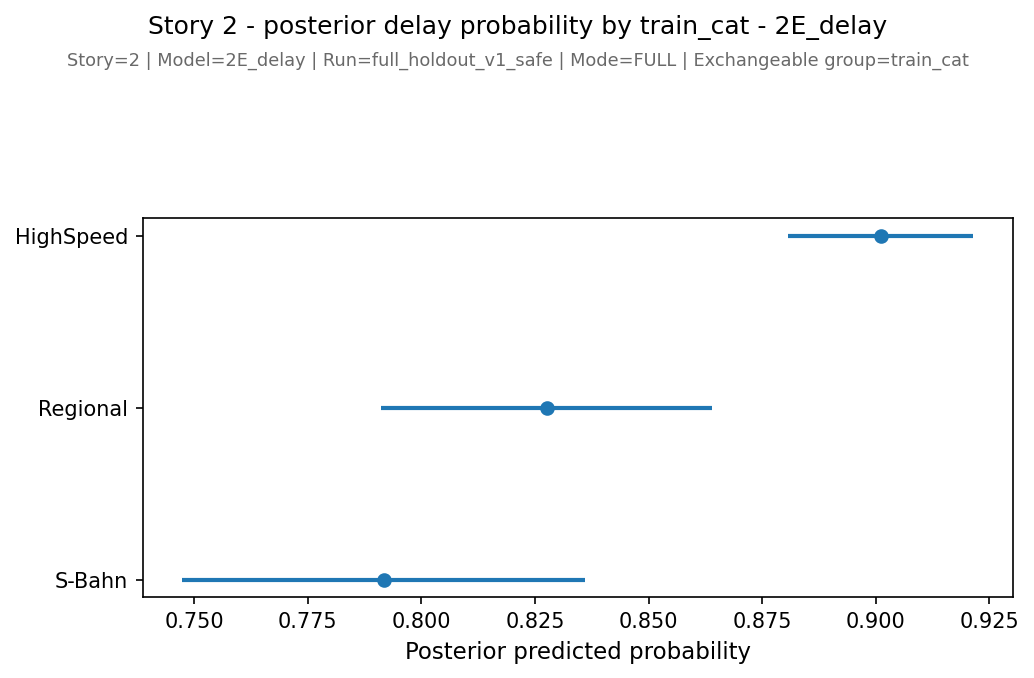
\includegraphics[width=0.72\textwidth]{../../outputs/ppc/story2_train_cat_probs_2E_delay.png}
    \caption{Posterior \texttt{train\_cat} probabilities for Story 2 event-level Bernoulli.}
    \label{fig:story2_prob_2E_appendix}
\end{figure}

\begin{figure}[htbp]
    \centering
    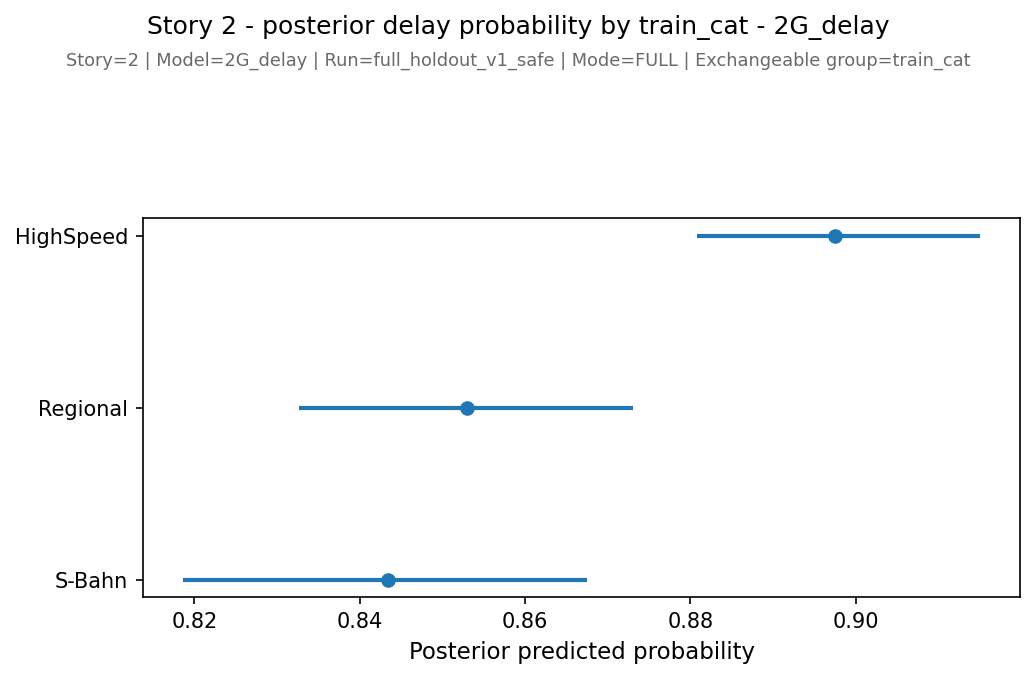
\includegraphics[width=0.72\textwidth]{../../outputs/ppc/story2_train_cat_probs_2G_delay.png}
    \caption{Posterior \texttt{train\_cat} probabilities for Story 2 grouped Binomial.}
    \label{fig:story2_prob_2G_appendix}
\end{figure}

\begin{figure}[htbp]
    \centering
    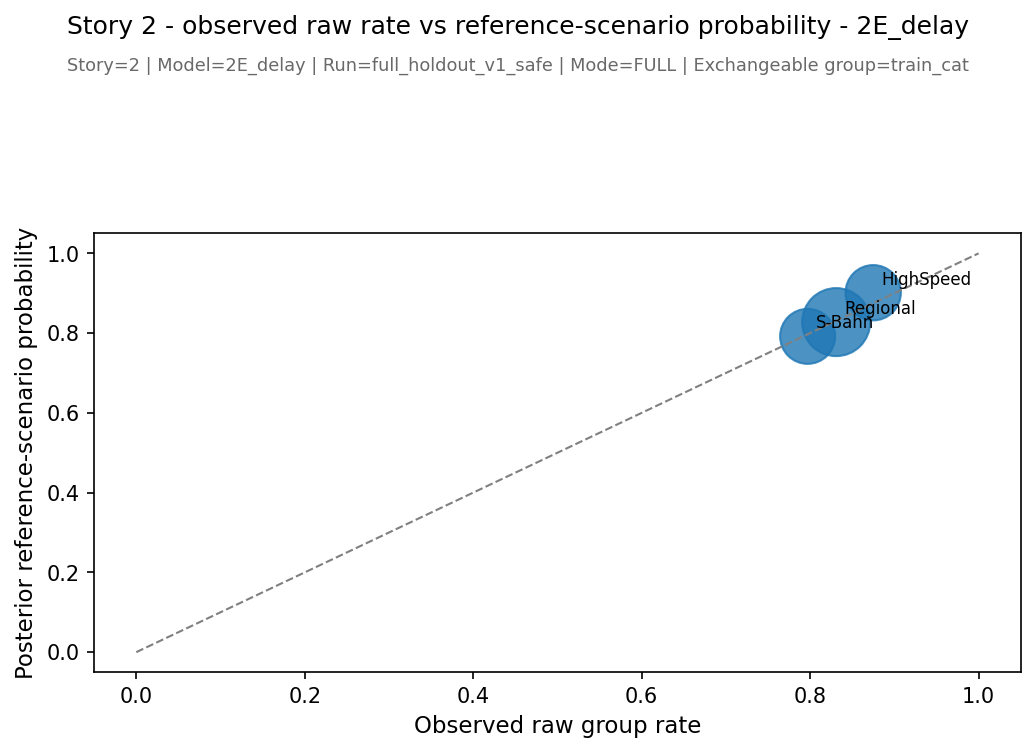
\includegraphics[width=0.72\textwidth]{../../outputs/ppc/story2_obs_vs_refprob_2E_delay.png}
    \caption{Observed raw rates versus reference-scenario posterior probabilities for Story 2 event-level Bernoulli.}
    \label{fig:story2_ref_2E_appendix}
\end{figure}

\begin{figure}[htbp]
    \centering
    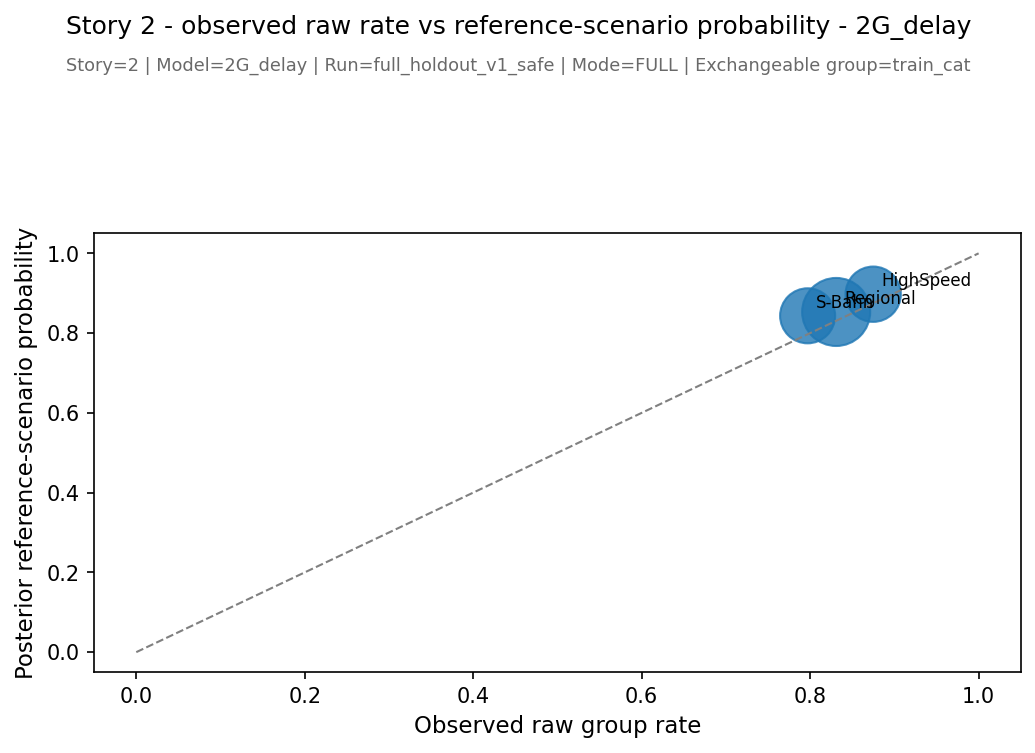
\includegraphics[width=0.72\textwidth]{../../outputs/ppc/story2_obs_vs_refprob_2G_delay.png}
    \caption{Observed raw rates versus reference-scenario posterior probabilities for Story 2 grouped Binomial.}
    \label{fig:story2_ref_2G_appendix}
\end{figure}

\FloatBarrier
\clearpage
\subsubsection*{Story 3}

\begin{figure}[htbp]
    \centering
    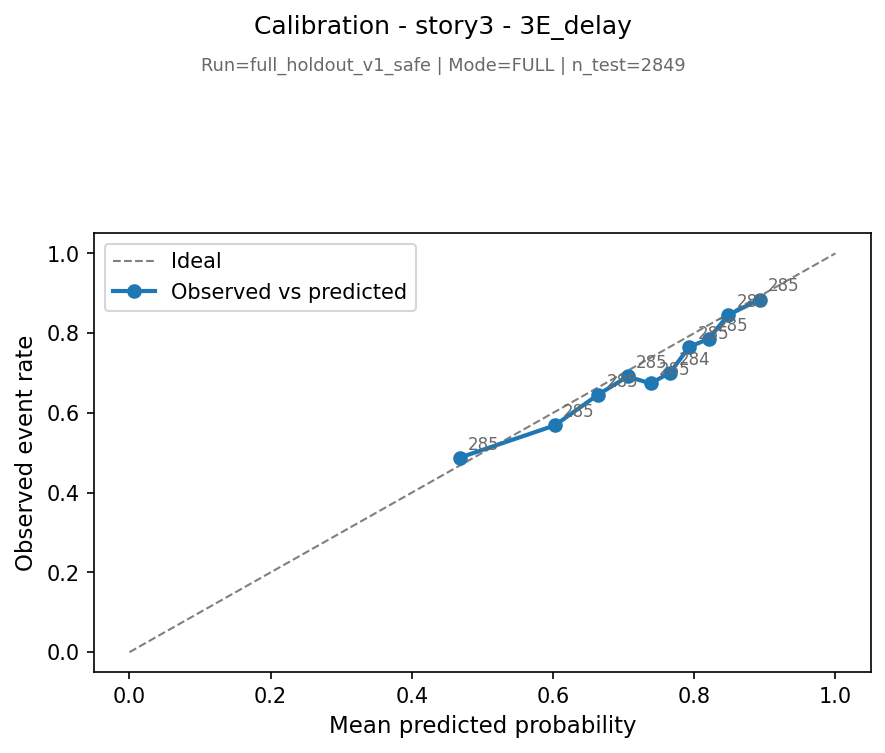
\includegraphics[width=0.72\textwidth]{../../outputs/ppc/story3_calibration_3E_delay.png}
    \caption{Calibration for Story 3 event-level Bernoulli.}
    \label{fig:story3_calib_3E_appendix}
\end{figure}

\begin{figure}[htbp]
    \centering
    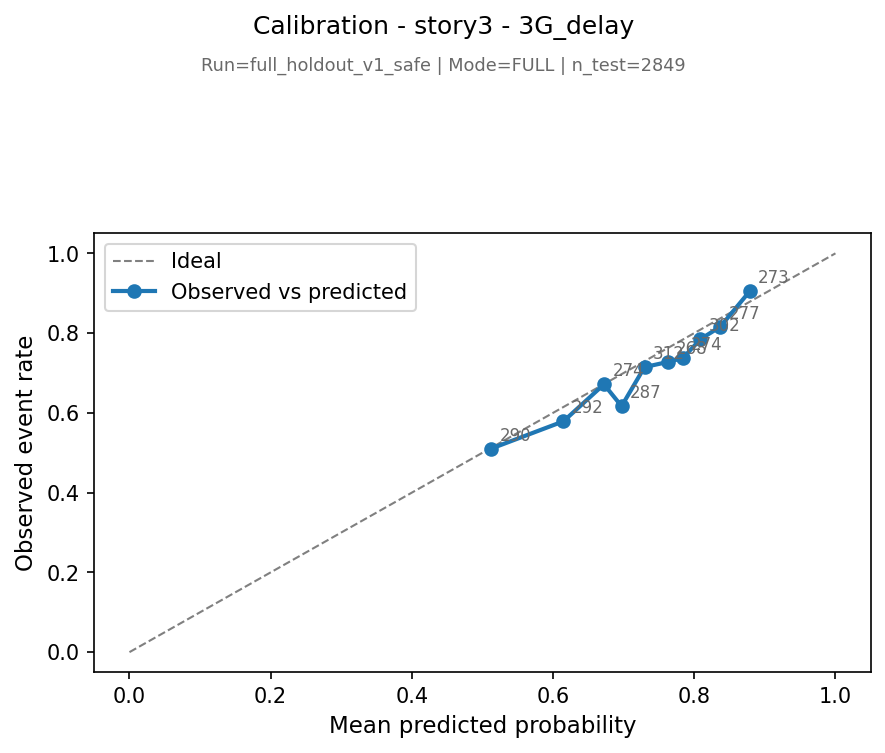
\includegraphics[width=0.72\textwidth]{../../outputs/ppc/story3_calibration_3G_delay.png}
    \caption{Calibration for Story 3 grouped Binomial.}
    \label{fig:story3_calib_3G_appendix}
\end{figure}

\begin{figure}[htbp]
    \centering
    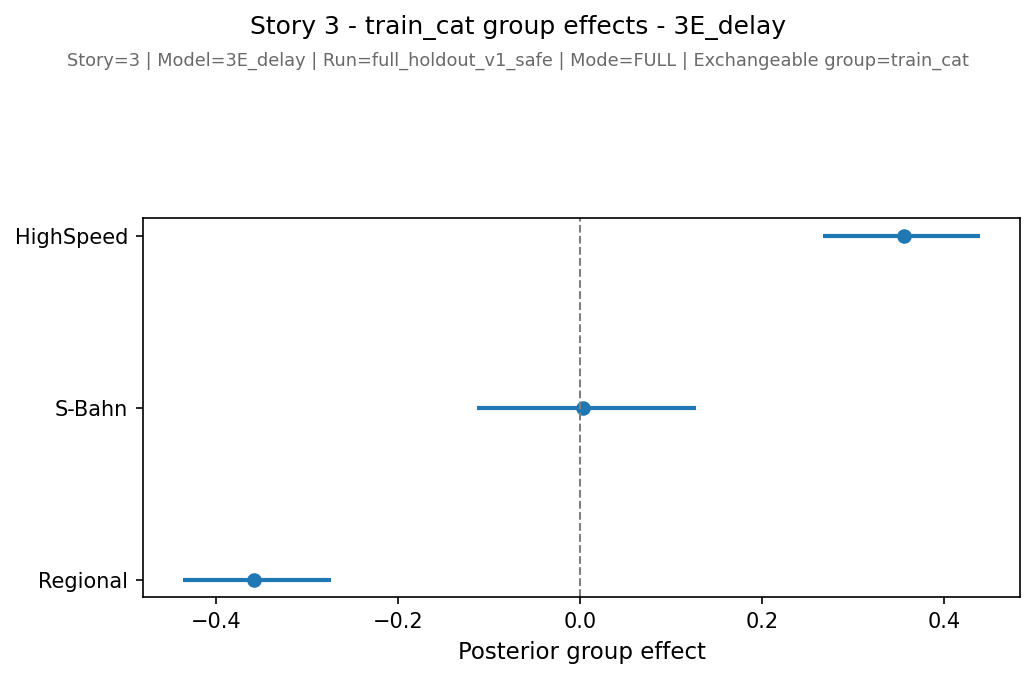
\includegraphics[width=0.72\textwidth]{../../outputs/ppc/story3_train_cat_effects_3E_delay.png}
    \caption{\texttt{train\_cat} effects for Story 3 event-level Bernoulli.}
    \label{fig:story3_eff_3E_appendix}
\end{figure}

\begin{figure}[htbp]
    \centering
    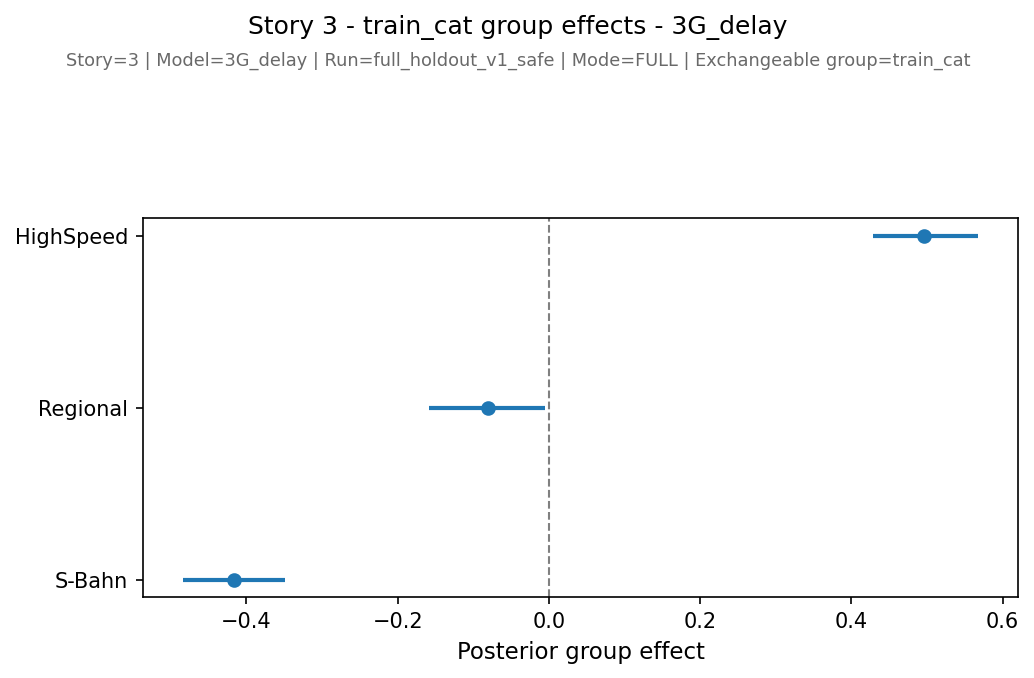
\includegraphics[width=0.72\textwidth]{../../outputs/ppc/story3_train_cat_effects_3G_delay.png}
    \caption{\texttt{train\_cat} effects for Story 3 grouped Binomial.}
    \label{fig:story3_eff_3G_appendix}
\end{figure}

\begin{figure}[htbp]
    \centering
    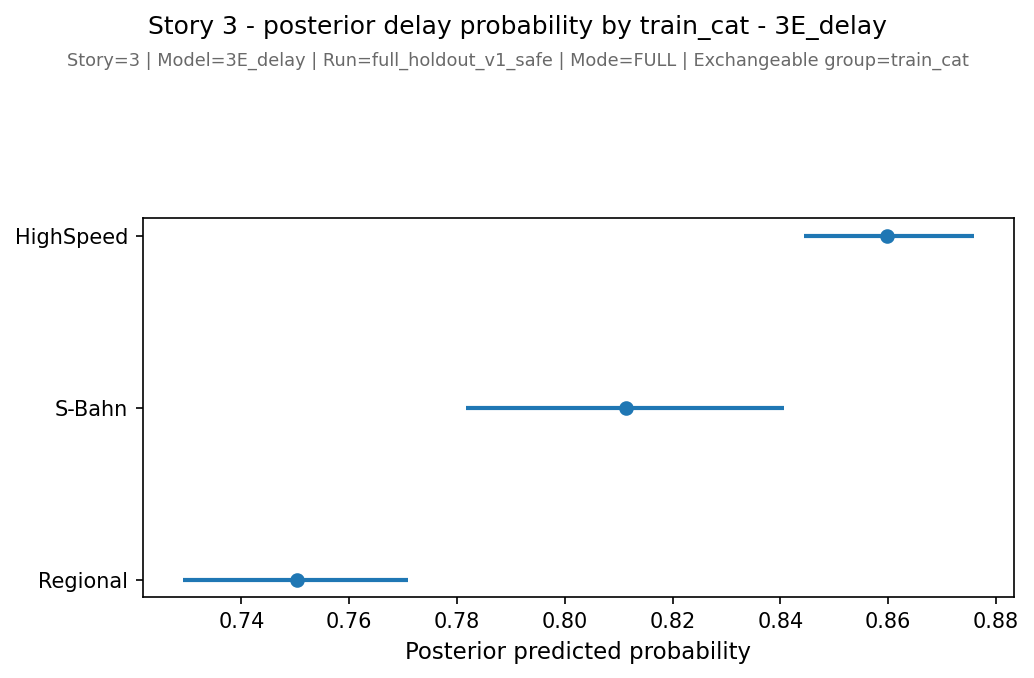
\includegraphics[width=0.72\textwidth]{../../outputs/ppc/story3_train_cat_probs_3E_delay.png}
    \caption{Posterior \texttt{train\_cat} probabilities for Story 3 event-level Bernoulli.}
    \label{fig:story3_prob_3E_appendix}
\end{figure}

\begin{figure}[htbp]
    \centering
    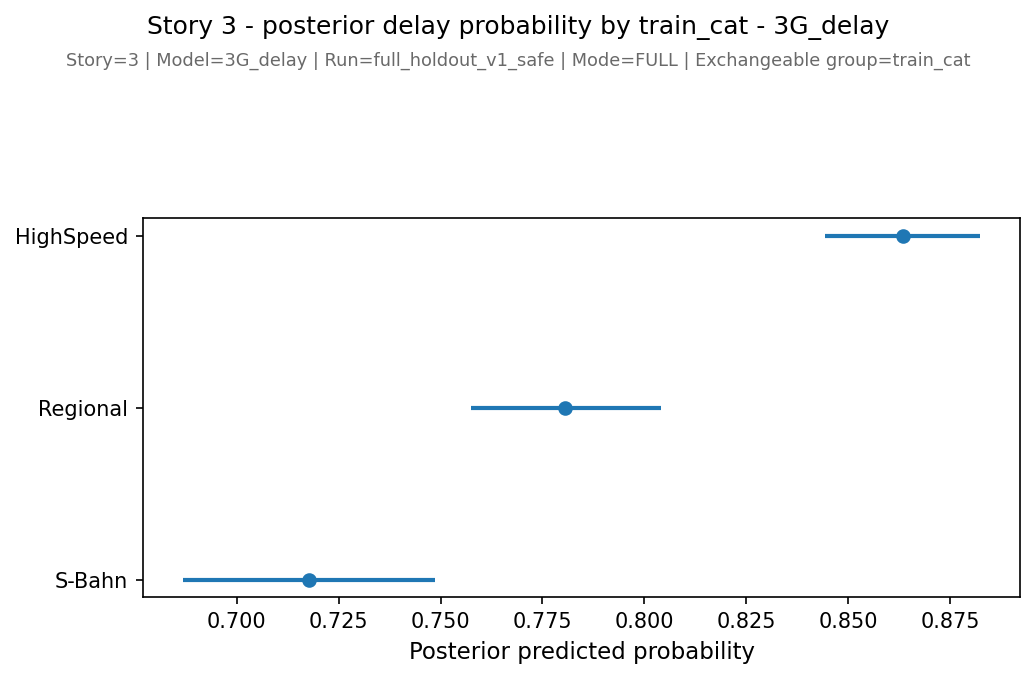
\includegraphics[width=0.72\textwidth]{../../outputs/ppc/story3_train_cat_probs_3G_delay.png}
    \caption{Posterior \texttt{train\_cat} probabilities for Story 3 grouped Binomial.}
    \label{fig:story3_prob_3G_appendix}
\end{figure}

\begin{figure}[htbp]
    \centering
    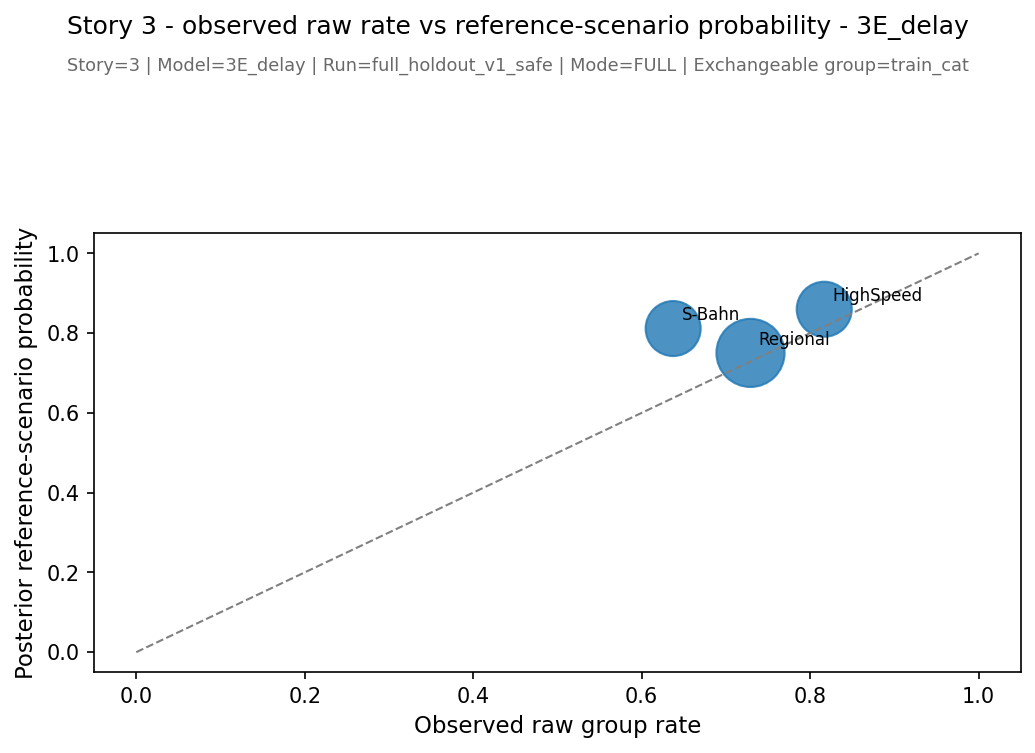
\includegraphics[width=0.72\textwidth]{../../outputs/ppc/story3_obs_vs_refprob_3E_delay.png}
    \caption{Observed raw rates versus reference-scenario posterior probabilities for Story 3 event-level Bernoulli.}
    \label{fig:story3_ref_3E_appendix}
\end{figure}

\begin{figure}[htbp]
    \centering
    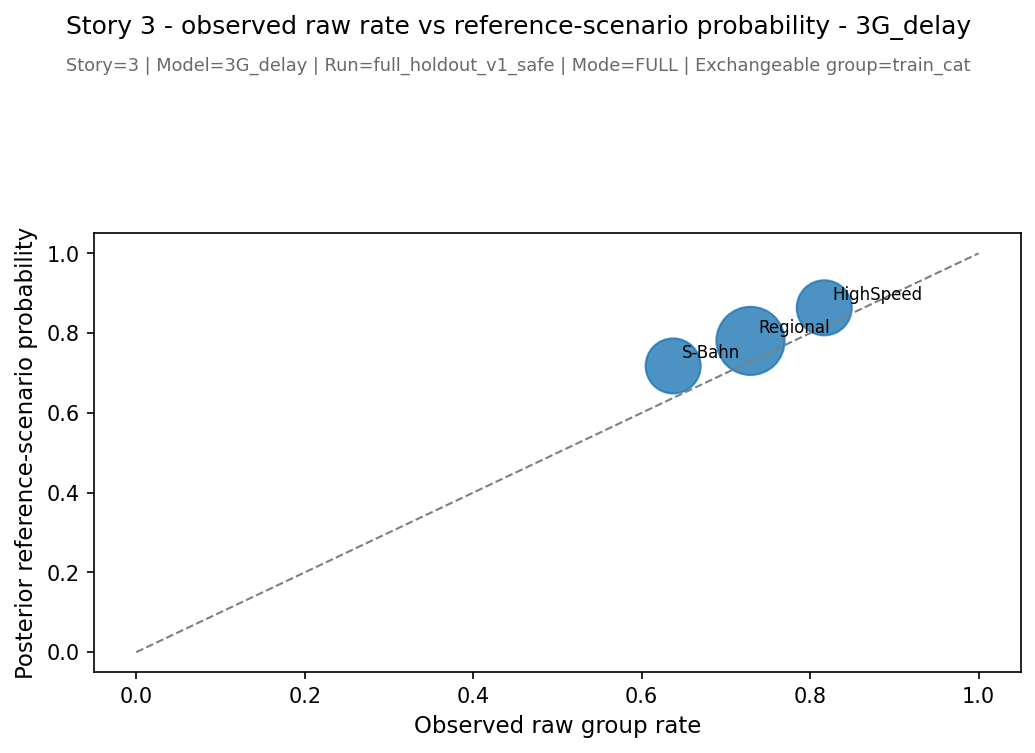
\includegraphics[width=0.72\textwidth]{../../outputs/ppc/story3_obs_vs_refprob_3G_delay.png}
    \caption{Observed raw rates versus reference-scenario posterior probabilities for Story 3 grouped Binomial.}
    \label{fig:story3_ref_3G_appendix}
\end{figure}

\FloatBarrier
\subsection{Additional output tables}
\label{sec:appendix_tables}
\FloatBarrier

In addition to the figures shown in the main text and appendix, the analysis pipeline produced supplementary output tables for convergence diagnostics, PSIS-LOO summaries, holdout comparison summaries, exchangeability summaries, grouped Binomial support data, and calibration values. These tables are included in the submitted output bundle and code archive but are not reproduced in full in the PDF report in order to keep the appendix readable.

\end{document}
